% !TEX Program = lualatex
\documentclass[11pt,
twoside,openright,    % for one-sided printing and screens
DIV=15,            % set the main text width
BCOR=8mm,         % binding correction
%parskip=half,      % enable if you want paragraphs separated by vertical spacing instead of indents
%draft              % enable to compile faster and test layout
]{scrreprt}
%\documentclass[report,mono,twoside,openright]{tugrazbooklet}
%\documentclass[a4paper]{book}

\usepackage[msc,nawi]{tugrazthesis}
% options:
%   - msc (for Master's thesis/Masterarbeit) OR
%     diplom (for Diploma thesis/Diplomarbeit) OR
%     phd (for Doctoral thesis/Dissertation)
%   - nawi (for NAWI curricula)
%   - individual (for Individuelles Masterstudium)




% Example packages for the dummy content
%info defined in shared preamble
\usepackage[ngerman,english]{babel}
\usepackage[utf8]{inputenc}
\usepackage{geometry}
\usepackage{microtype}
\usepackage[all]{nowidow}
\usepackage{tablefootnote}

%--- PREAMBLE ------------------------------------------------------------------
% <INSERT YOUR CUSTOM MACROS AND PACKAGES HERE>
\usepackage{iftex}

% text input and font
\ifluatex  % LuaLaTeX
    \usepackage{fontspec}
    % main font automatically: Latin Modern
    \IfFontExistsTF{Fira Code}{% true branch
        \setmonofont{Fira Code}[
            Contextuals=Alternate,  % Activate the calt feature
            StylisticSet={1,3,5,8}, % fontspec docs S. 46
            CharacterVariant={16}, % fontspec docs S. 37
            Numbers={SlashedZero} % fontspec docs S. 44
        ]}{% false branch
    }
\else  % pdfLaTeX
    \usepackage[utf8]{inputenc}  % input in UTF-8
    \usepackage[T1]{fontenc}  % output in T1 fonts (west European encoding)
    \usepackage{lmodern}  % Latin modern font for main text
    \IfFileExists{fira.sty}{% true branch
        \usepackage[mono]{fira}  % Fira (not Code!) font for monospaced text
    }{% false branch
    }
\fi

% text processing
\usepackage{babel}  % language package
\usepackage[intlimits]{mathtools}  % upgrade of amsmath (automatically loaded) - \int^_ like \limits^_
\usepackage{amssymb}  % upgrade of amsfonts (American Math Society)
\usepackage{amstext}  % \text command in math environments
\usepackage{letltxmacro}  % \let command for robust macros (new sqrt)
\usepackage{chemformula}  % typeset chemical formulas


% page geometry
\usepackage{scrlayer-scrpage}  % page formatting with KOMA options
% \usepackage[paper=a4paper, hmargin=3cm, vmargin=2.5cm, includehead, includefoot]{geometry}  % horizontal: 3cm, vertical: 2.5cm strict with or without headers and footers
\usepackage{tabto}  % tab stops
\NumTabs{8}  % 8 equally spaced of \textwidth tab stops



% floats
\usepackage[hypcap=false, labelfont=bf]{caption, subcaption}  % caption editing - hypcap warning with hyperref
% counter prefixed with section number and therefore reset at each section:
% \counterwithin{figure}{section}
% \counterwithin{table}{section}
\usepackage{float}  % for [H] (forced here) specifier
\usepackage{tabularray}  % better tables
\usepackage{caption}  % better captions


% graphical input
\usepackage{graphicx}  % input JPEG, PNG, PDF, etc.
\usepackage{pdfpages}  % input PDF as whole pages
\usepackage{lastpage}  % reference to last page
\usepackage{import} % include files from other directories


% text
\usepackage[locale=DE, uncertainty-mode=separate]{siunitx}  % SI units, German formatting - \pm stays \pm instead of ..(.)
% custom units:
\DeclareSIUnit{\hartree}{\ensuremath{E_{\mathrm{h}}}}

\let\sqty\qty  % physics overrides \qty of siunitx, therefore make it available as \sqty
\usepackage{physics}  % macros for easier typesetting of physical formulas
\usepackage{icomma}  % no space after commas instead of English points) in decimal values
\usepackage{enumitem}  % better enumerating with style options
\usepackage{nicefrac}  % inline-fractions in n/d-style
\usepackage{xcolor}  % custom colors
%TU-Graz colors
\definecolor{TUred}{HTML}{e4154b}
\definecolor{TUgray}{HTML}{bcbcbc}
\usepackage{listings, scrhack}  % code display; listings in combination with KOMA
\ifluatex
    \IfFontExistsTF{Fira Code}{%
        \usepackage[verbatim]{lstfiracode}  % Fira Code in listings
        \lstset{style=FiraCodeStyle}
    }{}
\fi
\usepackage{fancyvrb}  % Verbatim environment with better options (capital V!)


% literacy
\usepackage[sorting=none, giveninits=true, backend=biber]{biblatex}  % defaults: backend=Biber, style=numeric
% bibliography styles: https://www.overleaf.com/learn/latex/Biblatex_bibliography_styles
% citation styles: https://www.overleaf.com/learn/latex/Biblatex_citation_styles
\usepackage{csquotes}  % better quotation - should also be used in combination with package babel (warning)
\usepackage{xurl}  % breaks links - after BibLaTeX, but before hyperref!
\usepackage[hidelinks]{hyperref}  % produces most errors, last to load


% enumerate paragraphs and subparagraphs
% depths: https://www.overleaf.com/learn/latex/Sections_and_chapters
% -1 \part{part}
%  0 \chapter{chapter}
%  1 \section{section}
%  2 \subsection{subsection}
%  3 \subsubsection{subsubsection}
%  4 \paragraph{paragraph}
%  5 \subparagraph{subparagraph}
\setcounter{secnumdepth}{3}


% KOMA setups
% header and footer
\pagestyle{scrheadings}  % KOMA style
% \clearpairofpagestyles  % reset
% \setkomafont{pageheadfoot}{\normalfont}  % standard font in header and footer
% \setlength{\headheight}{27.2pt}  % warning
% \cfoot{\pagemark{}}  % centre foot - *: ref but no hyperlink
% {}: empty statement
% \ : protected space
% \,: small space
\DeclareTOCStyleEntry[linefill=\TOCLineLeaderFill]{tocline}{section}  % sections in TableOfContents with dotted lines
% source: https://tex.stackexchange.com/a/651532
\KOMAoptions{parskip=half-}  % paragraphs with half a line height space instead of indentation, last line with no special treatment


% package setups

% rewrite names (babel overwrites German with standard English names, therefore at document beginn [after everything is loaded])
\AtBeginDocument{\renewcommand{\refname}{Literaturverzeichnis}}
% others:
% \contentsname
% \listtablename
% \listfigurename

% make title in bibliography upright
\DeclareFieldFormat{title}{#1}  % https://tex.stackexchange.com/a/311837
% make size of url in bibliography smaller
\renewcommand{\UrlFont}{\footnotesize\ttfamily}  % https://tex.stackexchange.com/a/151115, https://www.overleaf.com/learn/latex/Font_sizes%2C_families%2C_and_styles


% xcolor
\definecolor{code_keyword}{HTML}{A06E9D}
\definecolor{code_string}{HTML}{AD6E3E}
\definecolor{code_comment}{HTML}{6A9955}
% \definecolor{keyword_pink}{HTML}{c678dd}
% \definecolor{vscode_bg}{HTML}{282c34}
% \definecolor{vscode_var}{HTML}{e06c75}
% \definecolor{vscode_comment}{HTML}{7f848e}
% \definecolor{vscode_constant}{HTML}{d19a66}
% \definecolor{vscode_function}{HTML}{61afe3}
% \definecolor{background_grey}{HTML}{f8f8f8}
% \definecolor{code_basic}{HTML}{D4D4D4}
% \definecolor{code_background}{HTML}{1E1E1E}

% custom siunitx units
\DeclareSIUnit{\dig}{dig}  % digits for uncertainty of electronical measurement devices
\DeclareSIUnit{\px}{px}  % pixels
\sisetup{detect-weight,
    mode=text,
    table-align-uncertainty=true,
        separate-uncertainty = false,
        multi-part-units = single,
        output-decimal-marker={.},}


% listings
\lstset{
    basicstyle=\ttfamily\footnotesize,%\color{code_basic},  % \footnotesize contains \selectfont implicitly
    %backgroundcolor=\color{code_background},
    commentstyle=\color{code_comment},
    keywordstyle=\bfseries\color{code_keyword},
    numberstyle=\tiny,
    stringstyle=\color{code_string},
    breakatwhitespace=false,
    breaklines=true,
    captionpos=b,
    keepspaces=true,
    numbers=left,
    numbersep=5pt,
    showspaces=false,
    showstringspaces=false,
    showtabs=false,
    tabsize=2
}


% new sqrt
% https://en.wikibooks.org/wiki/LaTeX/Mathematics
\makeatletter
\let\oldr@@t\r@@t
\def\r@@t#1#2{%
    \setbox0=\hbox{$\oldr@@t#1{#2\,}$}\dimen0=\ht0
    \advance\dimen0-0.2\ht0
    \setbox2=\hbox{\vrule height\ht0 depth -\dimen0}%
    {\box0\lower0.4pt\box2}}
\LetLtxMacro{\oldsqrt}{\sqrt}
\renewcommand{\sqrt}[2][\ ]{\oldsqrt[#1]{#2} }
\makeatother


% own commands
% \newcommand* can't contain multiple lines
% \newcommand can
\newcommand*{\mup}[1]{\ensuremath{\text{\textup{#1}}}}  % math mode upright normal font
\newcommand*{\inkgraphics}[3][\linewidth]{\def\svgwidth{#1}\import{#2}{#3}}


% custom tabularray environments

% imports and setups of tabularray: {
%     expl3,
%     xparse,
%     ninecolors
%     \hypersetup{pdfborder={0 0 0}}
% }

% additionally loaded libraries:
% diagbox
% varwidth
% booktabs
% counter

\UseTblrLibrary{amsmath}  % +array, +matrix, +bmatrix, +Bmatrix, +pmatrix, +vmatrix, +Vmatrix and +cases like tabularray with graphical options
\UseTblrLibrary{siunitx}  % siunitx suited for tabularray
\UseTblrLibrary{diagbox}  % table cells with diagonal lines, suited for tabularray
\UseTblrLibrary{varwidth}  % measure cell width
\UseTblrLibrary{booktabs}
\UseTblrLibrary{counter}


% custom tabularray environments:

% info:
% colcycle: https://github.com/lvjr/tabularray/issues/74
% guard: https://github.com/lvjr/tabularray/issues/175#event-6567229210

% guard S columns if latest feature ={guard} is not yet available
\newcommand*{\SiGuard}[1]{{#1}}

% standard environment
\SetTblrInner{
    hlines,
    vlines,
    columns={
            halign=c,
            valign=m,
        },
    measure=vbox,
}

% X columns
\NewTblrEnviron{tblrx}
\SetTblrInner[tblrx]{
    hlines,
    vlines,
    columns={
            halign=c,
            valign=m,
            co=1,  % coefficient of width for expendable columns (X columns)
        },
    width=\linewidth,
    vspan=minimal,
    measure=vbox,
}

% -X columns
\NewTblrEnviron{tblr-x}
\SetTblrInner[tblr-x]{
    hlines,
    vlines,
    columns={
            halign=c,
            valign=m,
            co=-1,  % shrinks X column down to natural width
        },
    width=\linewidth,
    vspan=minimal,
    measure=vbox,
}

% no hline and vline left and on top of first cell
\NewTblrEnviron{tblr_omit_first_cell}
\SetTblrInner[tblr_omit_first_cell]{
    hlines,
    vlines,
    columns={
            halign=c,
            valign=m,
        },
    hspan=even,
    vspan=minimal,
    %
    hline{1}={1}{white},  % first row, only first cell
    vline{1}={1}{white},
    measure=vbox,
}

% longtblr
\DefTblrTemplate{conthead-text}{default}{(Fortsetzung)}  % default: define and set at the same time
\DefTblrTemplate{contfoot-text}{default}{Fortsetzung auf nächster Seite}
\SetTblrStyle{caption-tag}{font=\bfseries}  % caption tag bold
\SetTblrInner[longtblr]{
    hlines,
    vlines,
    columns={
            halign=c,
            valign=m,
        },
    measure=vbox,
}

% longtblr - to adjust width of caption 
\DefTblrTemplate{firsthead}{default}{\addtocounter{table}{-1}\captionof{table}[\InsertTblrText{entry}]{\InsertTblrText{caption}}}
\DefTblrTemplate{middlehead,lasthead}{default}{\addtocounter{table}{-1}\captionof{table}[]{\InsertTblrText{caption}~(Fortsetzung)}}
%info ADD this to a local environment around the longtblr: \captionsetup{format=plain,labelfont=bf,font=small,  width=\linewidth}

\setlength{\parindent}{0pt}
\setlength{\parskip}{\baselineskip}

\newcommand{\bigO}[1]{\mathcal{O}\left(#1\right)}
\newcommand{\todo}[1]{\textbf{\textcolor{TUred}{#1\\}}}
\newcommand{\B}{\fontseries{b}\selectfont}


\addbibresource{thesis.bib}
\usepackage{adjustbox}
\usepackage{algorithm}
\usepackage{algpseudocode}
\usepackage{datetime}
\usepackage{tikz}
\usetikzlibrary{positioning, arrows.meta, shapes.multipart}
\usepackage[absolute,overlay]{textpos} % Enable absolute positioning\usepackage{datetime}
\usepackage{tocloft}
\usepackage{amssymb}

\usetikzlibrary{arrows}
\usetikzlibrary{positioning}

\providecommand{\algorithmautorefname}{Algorithm}
\renewcommand{\algorithmicrequire}{\textbf{Input:}}
\renewcommand{\algorithmicensure}{\textbf{Output:}}


\newcommand{\hrefu}[2]{\underline{\href{#1}{#2}}} % underline links
\newcommand{\TODO}[1]{\textcolor{red}{\textbf{TODO #1}}}

\begin{document}

%- Title ---
\def\mythesistitle{Machine Learning-Driven Initial Guess Prediction for SCF Procedures}
\def\mykeywords{computational physics, computational chemistry, machine learning, self-consistent field, initial guess prediction, GNN, graph neural network, density functional theory, DFT, quantum chemistry, QM9 dataset, electronic structure simulation, message passing neural network, message passing}
\def\mykeywordsabstract{computational quantum chemistry $\cdot$ density functional theory $\cdot$ graph neural network\\initial guess prediction $\cdot$ machine learning $\cdot$ self-consistent field}
\hypersetup{
  pdfauthor={Wachmann Elias},
  pdftitle={\mythesistitle},
  pdfkeywords={\mykeywords},
  pdfsubject={Master's Thesis},
  }

% Autoref with cap letters
\renewcommand{\subsectionautorefname}{Subsection}
\renewcommand{\sectionautorefname}{Section}
\renewcommand{\chapterautorefname}{Chapter}
\renewcommand{\figureautorefname}{Figure}
\renewcommand{\tableautorefname}{Table}
\renewcommand{\algorithmiccomment}[1]{\hspace{-1cm}\hfill$\triangleright$ \texttt{#1}}



\newdateformat{mydate}{\THEDAY\ \monthname[\THEMONTH]\ \THEYEAR}

%--- INFORMATION FOR TITLEPAGE -------------------------------------------------

% Your name including previous academic degrees (optional argument sets a different \author{}):
\thesisauthor[Elias Wachmann]{Elias Wachmann, BSc. BSc.}

% Title of your thesis (optional argument sets a different \title{}):
\thesistitle{\mythesistitle}

% Date of completion (optional argument sets a different \date{})
\thesisdate[ ]{\monthname\ \the\year}

% Supervisor headline (select male/female/plural version)
\supervisortitle{\germanenglish{Betreuerin/Betreuer}{Supervisor}}

% Supervisor info
\supervisor{%
  Assoc.Prof. Mag.phil. Dipl.-Ing. Dr.phil. Dr.techn. Andreas Hauser\\
  \medskip
  Institute of Experimental Physics
}
\cosupervisortitle{\germanenglish{Betreuerin/Betreuer}{Co-Supervisor}}
\cosupervisor{
  Dipl.-Ing. Dr.techn. Ralf Meyer, BSc\\
  \medskip
  Institute of Experimental Physics}

% Academic degree achieved with this thesis, according to your curriculum (check curriculum and select male/female version):
\academicdegree{Diplom-Ingenieur}
% 
%\academicdegree{Master of Science} % msc
%\academicdegree{Diplom-Ingenieur/Diplom-Ingenieurin} % msc
%\academicdegree{Magister/Magistra der Naturwissenschaften} % diplom
%\academicdegree{Doktor/Doktorin der technischen Wissenschaften} % phd
%\academicdegree{Doktor/Doktorin der Naturwissenschaften} % phd
%\academicdegree{Master of ???} % individual

% Name of your degree programme according to your curriculum (only for msc/diplom; status of the list: academic year 2019/20)
\curriculum{Technical Physics } % 486

\pagenumbering{roman}
\printthesistitle


  %--- FRONT MATTER --------------------------------------------------------------
\newcommand{\textfield}[2]{
  \vbox{
    \hsize=#1\kern3cm\hrule\kern1ex
    \hbox to \hsize{\strut\hfil\footnotesize#2\hfil}
  }
}


\clearpage
\section*{Affidavit}
I declare that I have authored this thesis independently, that I have
not used other than the declared sources/resources, and that I have
explicitly indicated all material which has been quoted either
literally or by content from the sources used. The text document
uploaded to \textsc{TUGRAZ}online is identical to the present bachelor's
thesis.

\setlength{\TPHorizModule}{1mm}
\setlength{\TPVertModule}{1mm}
\begin{textblock}{3}(108,85)
  % \includegraphics[scale=2]{fig/affidavit/signature_transparent.png}
\end{textblock}
\begin{textblock}{50}(28,89)
  \begin{center}
    \mydate\today
  \end{center}
\end{textblock}

\hbox to \hsize{\textfield{4cm}{Date}\hfil\hfil\textfield{7cm}{Signature}}
% }{
%   \section*{Eidesstattliche Erklärung}
%   \foreignlanguage{ngerman}{%
%     Ich erkläre an Eides statt, dass ich die vorliegende Arbeit
%     selbstständig verfasst, andere als die angegebenen
%     Quellen/Hilfsmittel nicht benutzt, und die den benutzten Quellen
%     wörtlich und inhaltlich entnommenen Stellen als solche kenntlich
%     gemacht habe. Das in \myacro{TUGRAZ}online hochgeladene Textdokument
%     ist mit der vorliegenden Dissertation identisch.}

%     \hbox to \hsize{\textfield{4cm}{Datum}\hfil\hfil\textfield{7cm}{Unterschrift}}
% }

\newpage
\chapter*{Abstract}

\paragraph{Keywords:}
computational physics $\cdot$
\TODO{}
\chapter*{Kurzfassung}


\TODO{Wie Abstract nur direkt auf deutsch übersetzt.}
\chapter*{Acknowledgements}
\label{chap:acknowledgements}

I am profoundly thankful to Prof. Andreas W. Hauser and Ralf Meyer for letting me choose a topic dear to my heart and giving me the freedom to explore it in my own way. Their guidance and support were invaluable throughout this journey.

I also want to express my appreciation towards the rest of our group, especially Dominik, for the many insightful conversations we shared. A special thanks go to Nadja, for her thoughtful critiques and editorial support. To all my friends and colleagues, your support means the world to me and made stressful times much more bearable. My sincere gratitude goes to the Fürst Dietrichstein'sche Stiftung for their scholarship and the Institute of Experimental Physics for funding my master's thesis.

I would like to extend my heartfelt thanks to my parents, who always supported me unconditionally throughout my studies. Their encouragement and belief in me have been a constant source of motivation. 
\clearpage

% Roman page numbers for front matter

\setlength{\cftbeforesecskip}{3pt} % adjust as needed
\setlength\cftparskip{-2pt} % adjust as needed

\tableofcontents

% Switch to arabic page numbers, starting from 1
\cleardoublepage
\pagenumbering{arabic}


\chapter{Introduction}
\label{sec:introduction}

\chapter{Background}
\label{sec:background}

%! Editing first round done + spelling!
\chapter{Fock Matrix prediction}
\label{chap:fock_matrix_predictions}

SCF methods initially need a density matrix to start off their iterative calculations. Regardless of how the initial guess is chosen, the computational effort of this step should be negligible compared to the actual SCF iterations.\\
As a first step, we will introduce a method by which the density matrix is constructed from the Fock matrix. The latter is the target for various regression and MLP models which will be introduced in the subsequent sections.


\section{Introduction}
\label{sec:Fock_mathcalrix_prediction_intro}
As explained in \autoref{subsec:background_hf_computational}, the density matrix $P$ is calculated from the coefficient matrix $C$, which is obtained from the eigenvalue problem of the Fock matrix $F$:
\begin{equation}
    \label{eq:density_reconstruction_from_fock}
    F(P)\,C = SC\varepsilon \rightarrow P = 2\,\sum_{i}^{n_{occ}} C_{\mu i}\,C^*_{\nu i}\,,%2CC^T
\end{equation}

\begin{figure}[H]
    \centering
    \begin{tikzpicture}[scale=1, every node/.style={transform shape}]
        \def\imgwidth{0.30\linewidth}
        
        \node[anchor=south west, inner sep=0] (img1) at (0,0)
        {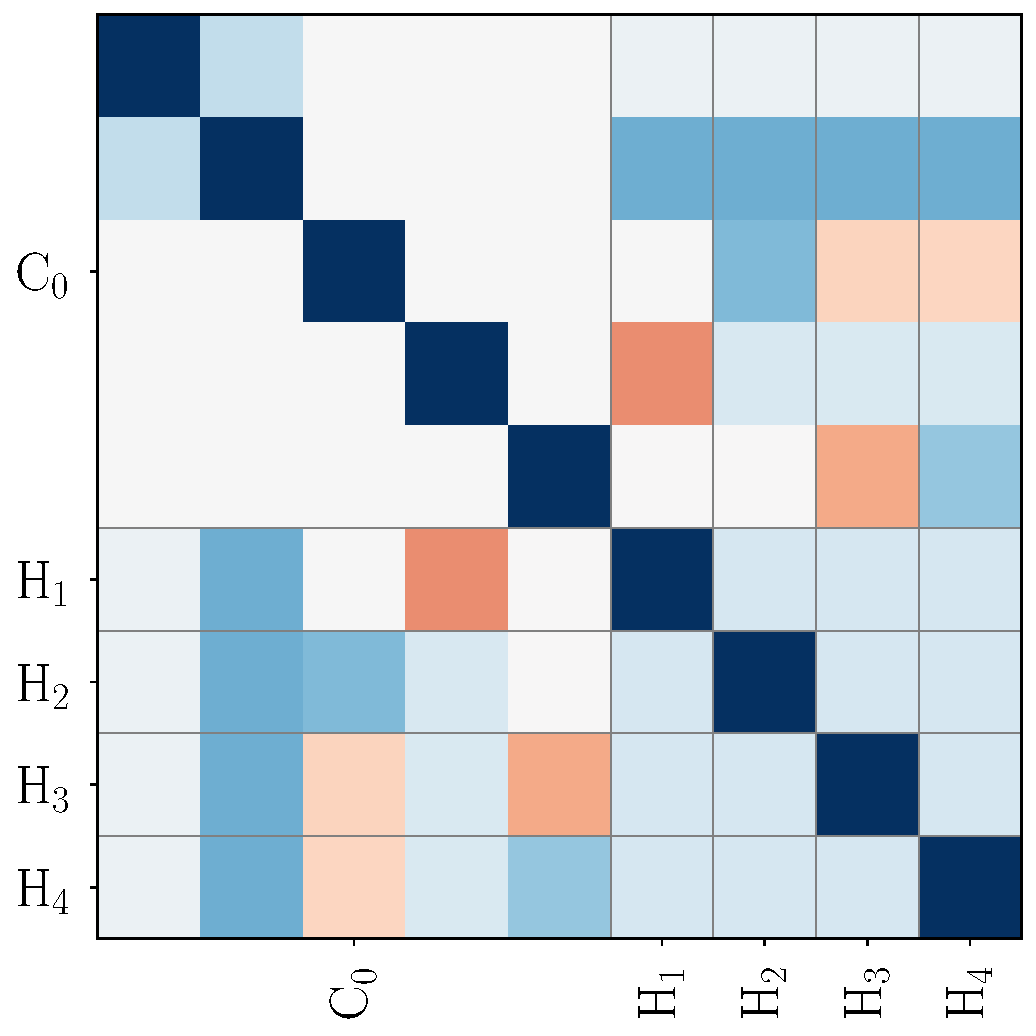
\includegraphics[width=\imgwidth]{../fig/c5h4n2o2/overlap_dsgdb9nsd_000001.pdf}};
        \node[above=2pt of img1.north, anchor=south, font=\small, xshift=10pt] {Overlap};
        
        \node[anchor=south west, inner sep=0] (img2) at (5.1,0)
        {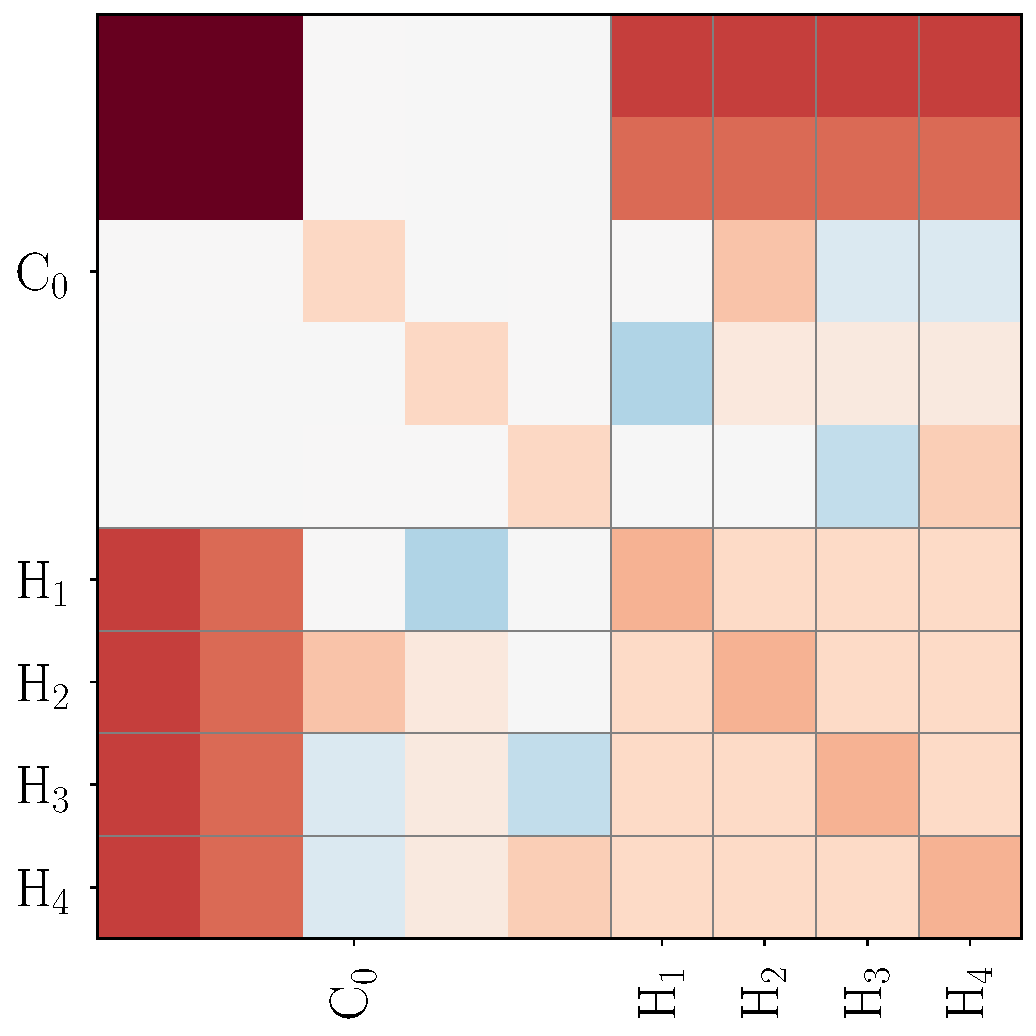
\includegraphics[width=\imgwidth]{../fig/c5h4n2o2/fock_dsgdb9nsd_000001.pdf}};
        \node[above=2pt of img2.north, anchor=south, font=\small, xshift=10pt] {Fock};
        
        \node[anchor=south west, inner sep=0] (img3) at (10.2,0)
        {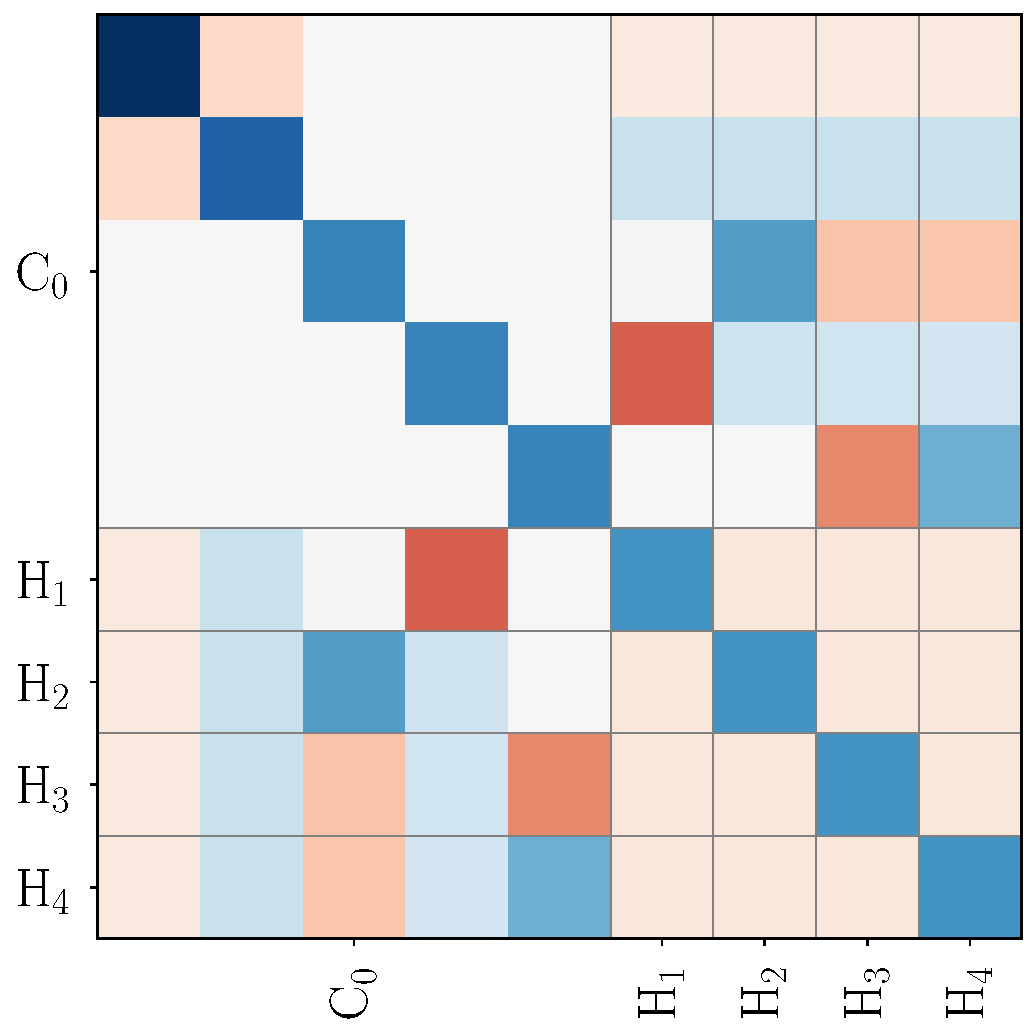
\includegraphics[width=\imgwidth]{../fig/c5h4n2o2/density_dsgdb9nsd_000001.pdf}};
        \node[above=2pt of img3.north, anchor=south, font=\small, xshift=10pt] {Density};
        
        \draw[->, thick] (4.3,2.4) -- node[above, align=center, font=\tiny]{ML\\model} (5.2,2.4);
        \draw[->, thick] (9.4,2.4) -- node[above, font=\tiny, yshift=1pt]{$P{=}2CC^{\mathrm{T}}$} (10.3,2.4);
    \end{tikzpicture}
    \caption[Schematic overview data flow]{Schematic overview of the data flow (using \ch{CH4}): overlap matrix to Fock matrix via ML model prediction, and construction of the density matrix from the Fock matrix.}
    \label{fig:method_data_flow}
\end{figure}
Effectively, one performs part of the SCF cycle here to obtain the density matrix, which ideally should be close to the final density matrix. This step takes $\bigO{N^3}$ time, which is asymptotically faster than $\bigO{N^4}$ time of the SCF cycles. 

The schematic workflow for the generation of a density matrix from the overlap matrix is shown in \autoref{fig:method_data_flow}. Overlap and density matrices appear visually similar, which might lead to the conclusion that predicting the density matrix directly from the overlap matrix is easier. However, learning the Fock matrix tends to involve fewer strict physical constraints. A Fock matrix primarily needs to be Hermitian, while a density matrix must be strictly positive semidefinite by construction, as well as normalized to the correct number of electrons. That makes direct density matrix learning more challenging, whereas learning the Fock matrix and then obtaining the density through diagonalisation could yield better results. We shall investigate this hypothesis in the following experiments.\\

Additionally, reconstructing the density from the Fock matrix amplifies residual errors in the predicted Fock matrix, since the density arises from a self-consistent eigenproblem involving both $F$ and $S$. Ideally, such errors should be small enough to not significantly affect the subsequent SCF iterations. In practice, some iterations (2-5) are always needed, even if we try to run the calculation with a guessed density constructed from the converged $F$ \& $S$ matrices.\\

\section{\ch{C5H4N2O2}-subset: A first trial}
\label{sec:qm9_c5h4n2o2}

As a proof of concept we will use 508 constitutional isomers\footnote{From the 509 constitutional isomers of \ch{C5H4N2O2} 508 converged using the STO-3G basis and the B3LYP functional.} of \ch{C5H4N2O2} from the QM9 dataset. 
Single point RKS simulations in \textsc{PySCF} \parencite{ref:pyscf} were performed for these molecules using the B3LYP\footnote{B3LYPG was used to be consistent with the Gaussian program package} functional and the STO-3G basis. The resulting converged density-, fock-, and overlap-matrices were saved for future training purposes. For our very minimal basis, these matrices are of size $49 \times 49$ as can be seen for a converged density in \autoref{fig:density_dsgdb9nsd_022700}. 
Due to the symmetry of the matrices we can discard nearly half of the elements and are left with 1225 features to learn. A rule of thumb for training classical statistical models is to have at least 10 samples per feature. \parencite{ref:rule_of_10} The given dataset of 508 samples is therefore far from this rule if we discard multiplicity in atoms in the samples. As a first step we shall limit our efforts to single models predicting the system based on the full overlap matrix. Nevertheless, the row / column order of our atoms in the overlap matrix has to be consistent for all the samples in the dataset (as seen in \autoref{fig:density_dsgdb9nsd_022700}). This is achieved by sorting the atoms in the overlap matrix according to their atomic number. Now we are ready to start off our endeavour with a Ridge regression model as a first trial. 

\begin{figure}[H]
    \centering
    \includegraphics[width=\textwidth]{../fig/c5h4n2o2/density\_dsgdb9nsd\_022700.pdf}
    \caption[Density matrix of dsgdb9nsd\_022700 in the STO-3G basis with theory level B3LYP]{Converged density of dsgdb9nsd\_022700 in the STO-3G basis with theory level B3LYP. The density matrix is of size $49 \times 49$ and is symmetric. The diagonal elements in the shown AO basis correspond to Mulliken AO-populations. }
    \label{fig:density_dsgdb9nsd_022700}
\end{figure}


\section{Ridge Regressor model} % updated with new sorted dataset
\label{sec:ridge_regressor_model}
The Ridge Regressor (RR) is set up with a typical $80 / 20$ train/test split. Overlap (input) as well as Fock (output) matrices are flattened and overlap (input) matrices are additionally rescaled using the \textsc{scikit-learn}'s default Standard Scaler. \parencite{ref:sk-learn} Using a 5-fold cross validation the model, a Multi-Output-Regressor is trained \footnote{also using \textsc{scikit-learn}'s \textsc{RidgeCV} and \textsc{MultiOutputRegressor} classes} with 10 equally $\log_{10}$-spaced $L^2$-regularization parameter $\alpha$ values ranging from $10^{-2}$ to $10^{3}$. Subsequently, the model is retrained with the arithmetic mean of the best performing $\alpha$ values ($\alpha_{\text{mean}} \approx 34$). This averaging reduces overfitting and yields a slightly lower RMSE on the test set compared to using individual $\alpha$ values per regressor. %! Note the averaging actually leads to a lower RMSE in test set compared to non-averaging the multi-regressor Model!  test RMSE 0.03231 vs. 0.03228 (averaging)
For the Fock matrix prediction the model yields a RMSE of $0.0057$ on the training set and $0.032$ on the test set which indicates overfitting of the model. We obtain the results in \autoref{tab:ridge_metrics} for the model and various guessing schemes implemented in \textsc{PySCF} (guessing schemes implemented in \textsc{PySCF} are listed in \autoref{sec:pyscf_initial_guessing_methods}).

\begin{table}[h]
    \centering
    \caption[\ch{C7H10O2} subset - iterations to convergence Ridge regression]{Comparison of different guessing schemes for 102 (20\%) test samples from the \ch{C5H4N2O2} subset from QM9 \parencite{ref:article1_qm9}. The average F-score is calculated on the test set using the Fock matrix prediction from the Ridge regression model and various guessing schemes implemented in \textsc{PySCF}. Additionally, we report the average number of iterations to convergence and the inference time, expressed relative to the inference time of the \texttt{minao} guess. The line `Not-converged' represents the percentage of samples not converging within 50 iterations.}
    \label{tab:ridge_metrics}
    \resizebox{\textwidth}{!}{
    \begin{tabular}{l
                    S[table-format=1.2(2)]
                    S[table-format=1.3(3)]
                    S[table-format=1.2(2)]
                    S[table-format=1.3(3)]
                    S[table-format=1.3(3)]
                    S[table-format=1.3(3)]}
        \toprule
        \textbf{Method} & \texttt{Ridge-model} & \texttt{minao} & \texttt{1e} & \texttt{atom} & \texttt{hückel} & \texttt{vsap} \\
        \midrule
        F-score / 1 & 0.93 \pm 0.04 & 0.899 \pm 0.002 & 0.71 \pm 0.02 & 0.802 \pm 0.0010 & 0.840 \pm 0.010 & 0.993 \pm 0.002 \\
        Iterations / 1 & 14 \pm 3 & 11.7 \pm 1.0 & 23 \pm 4 & 11.4 \pm 0.8 & 22 \pm 6 & 12.8 \pm 1.1 \\
        Inference-speed / 1 & 0.7 \pm 0.3 & 1.0 &  0.05 \pm 0.02 & 0.5 \pm 0.4 & 0.5 \pm 0.3 & 3 \pm 1.3 \\
        Not-Converged / \% & 4 & 0 &  31 & 0 & 27 & 0\\
        \bottomrule
    \end{tabular}
    }
\end{table}
Ridge regression performs better than the \texttt{1e} and \texttt{hückel} guessing schemes in terms of iterations, but still fares worse in comparison to the \texttt{minao}, \texttt{atom} and \texttt{vsap} guessing schemes. It should be noted that there seems to be no significant correlation of the F-score with the number of iterations till convergence. While \texttt{vsap} yields by far the highest F-score, it takes on average one iteration more to converge than the \texttt{minao} guessing scheme. This hints at the fact that some guessing strategies might guess better in regions in the density matrix which are more relevant for convergence speed than others. \\
Comparing the normalized difference to the reference density for the 102 test sample for \texttt{minao}, \texttt{vsap} and the Ridge regression model in \autoref{fig:density_error_comparison} gives different error patterns.  

\begin{figure}[H]
    \centering
    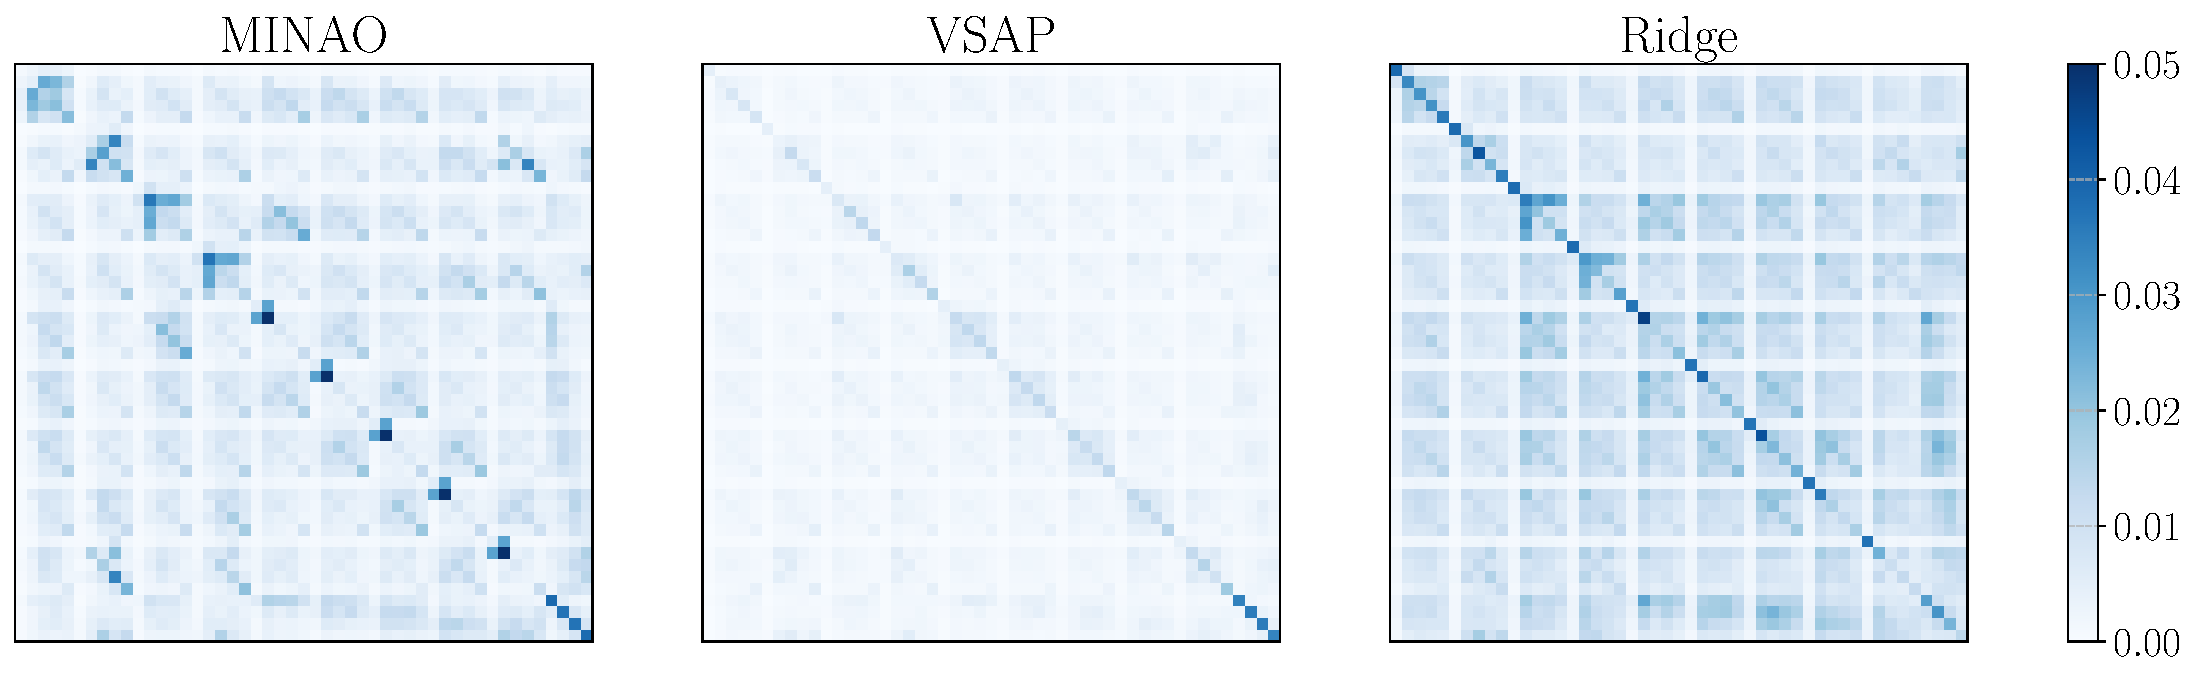
\includegraphics[width=\textwidth]{../fig/c5h4n2o2/density_error_comparison.pdf}
    \caption[Normalized difference of density guesses]{Normalized mean absolute difference of $\alpha$-electron density guesses to their converged density for \texttt{minao} \& \texttt{vsap} guess and the Ridge regression model evaluated on the test set: 102 (20\%) test samples from the \ch{C5H4N2O2} subset from QM9 \parencite{ref:article1_qm9}.}
    \label{fig:density_error_comparison}
\end{figure}
All three guessing schemes have spots on the main diagonal of the density matrix, where they are likely to differ from the reference solution. Interestingly, a Mulliken population analysis (see \autoref{subsec:background_hf_derived_quantities}) \parencite{ref:Mulliken_population_analysis} yields a mean value of $31.766$ on the test set prediction for \texttt{minao}, while \texttt{vsap} yields $32$ (only $\alpha$-electrons), as expected. A small error in the initial guess doesn't slow down convergence, since the self-consistent cycle corrects it right away. Comparing \texttt{minao} and \texttt{vsap} with our Ridge Model, the later fares worse on the main diagonal, especially for p-Orbitals. While \texttt{minao} exhibits more pronounced off-diagonal noise in comparison to \texttt{vsap}, this does not seem to affect convergence speed. At least for this small basis set, errors in the off-diagonal elements do not appear to hinder fast convergence.\\
% From that we might conclude that a good guess should be close to the reference density especially on the main diagonal, but not necessarily in the off-diagonal elements. We shall continue to investigate this in the next section.

\section{Kernel Ridge Regression}
\label{sec:kernel_ridge_regression}
Our baseline Ridge Regression (RR) model already introduced $L^2$-regularization handling collinearity which is doomed to happen in our dataset. However, it only models linear relationships between our input and output features. Kernel Ridge Regression (KRR) extends this by using kernel functions to generate a mapping from the input space via a higher dimensional feature space to the output space. This allows nonlinear relationships to be learned. \\
Using the same train/test split as before, we fit a KRR model with three different kernels: RBF, polynomial of degree 2 and polynomial of degree 3. 
Rather than averaging per-target $\alpha$ values (like in the RidgeCV above), we use a joint BayesSearch with 5-fold cross validation and 30 iterations\footnote{Hyperparameters see \autoref{tab:kernel_ridge_hyperparams}} to obtain the results in \autoref{tab:kernel_ridge_metrics}.

\begin{table}[h]
    \centering
    \caption[\ch{C7H10O2} subset - iterations to convergence Kernel Ridge regression]{Comparison of different Kernel Ridge regression (KRR) guessing schemes for 102 (20\%) test samples from the \ch{C5H4N2O2} subset from QM9 \parencite{ref:article1_qm9}. The F-score is calculated using the Fock matrix prediction from the Kernel-Ridge regression model and the \texttt{minao} guess. The number of iterations until convergence is shown, as well as the percentage samples not converging within 50 iterations and the inference time as a factor of the inference time of the \texttt{minao} guess.}
    \label{tab:kernel_ridge_metrics}
    \resizebox{\textwidth}{!}{
        \begin{tabular}{l
                        S[table-format=1.2(2)]
                        S[table-format=1.3(3)]
                        S[table-format=1.2(2)]
                        S[table-format=1.3(3)]}
            \toprule
            \textbf{Method} & \texttt{KRR RBF} & \texttt{KRR quadratic poly} & \texttt{KRR cubic poly} & \texttt{minao} \\
            \midrule
            F-score / 1         & 94 \pm 4 & 94 \pm 4 & 53 \pm 1.5 & 0.899 \pm 0.002 \\
            Iterations / 1      & 14 \pm 3 & 14 \pm 3 & 20 \pm 5 & 11.7 \pm 1.0 \\
            Inference-speed / 1 & 30 & 20 & 19 & 1.0\\ %! This is obviously very amusing in terms of uncertainty (therefore no uncertainty here)
            Not-Converged / \%  & 4 & 4 & 12 & 0\\
            \bottomrule
        \end{tabular}
    }
\end{table}
Hyperparameters found by the BayesSearch are shown bellow in \autoref{tab:kernel_ridge_hyperparams}.

\begin{table}[h]
        \centering
    \caption[Hyperparameter Kernel Ridge regression]{Hyperparameters found using BayesSearch for the Kernel Ridge regression models with different kernels.\\Search space: $\alpha \sim \operatorname{LogUniform}(10^{-8},10^{4})$, $\gamma \sim \operatorname{LogUniform}(10^{-6},10^{3})$ and $\mathrm{coef0} \sim \operatorname{Uniform}(0,1)$ for polynomial kernels; for the RBF kernel $\mathrm{coef0}$ is ignored}
    \label{tab:kernel_ridge_hyperparams}
    \begin{tabular}{l
                    S[table-format=1.0e1]
                    S[table-format=1.1e1]
                    S[table-format=1.1e1]}
        \toprule
        \textbf{Hyperparameter} & \texttt{KRR RBF} & \texttt{KRR quadratic poly} & \texttt{KRR cubic poly}\\
        \midrule
        $\alpha$ & 2e-8 & 1e-8 & 5e-2 \\
        $\gamma$ & 4e-5 & 7e-5 & 1e-6 \\
        $\mathrm{coef0}$ & \text{-} & 7.5e-1 & 1.4e-1 \\
        \bottomrule
    \end{tabular}
\end{table}

While RBF and quadratic kernels yield nearly comparable results, with the exception of inference speed, the cubic kernel performs significantly worse. The underperformance of the cubic kernel can be explained by the fact that the Bayes search gave a relatively high $\alpha$ value of $0.05$, which leads to a strong regularization of the model, making it less flexible. Even with lower regularization the cubic kernel, as well as the other two kernels, does not yield comparable performance to the \texttt{minao} guessing scheme. Interestingly, our models yield a significantly higher F-score (exception: cubic kernel) compared to \texttt{minao} but take more iterations to converge. A pattern which we have seen before with the Ridge regression model emerges again. This and the inefficient scaling of KRR with the number of samples lead us to explore different approaches in the next section.\\ 



\section{Further trials using MLP}
\label{sec:further_trials_mlp}
Previously, we tried to learn a mapping from overlap to Fock matrix solely via machine learning means. We have established that the quality for these guesses even on the minimal STO-3G basis is not on par with the established guessing schemes.\\
Predicting the main diagonal for a given system is an easier target, given the fact that the model predicts $N$ features from the $N^2$ input features. One established way of constructing the off diagonal elements is the generalized Wolfsberg-Helmholtz (GWH) construction \parencite{ref:gwh_wolfsberg1952spectra} (see \autoref{eq:gwh}).
Utilizing this construction on our dataset we obtain comparable results to our base Ridge regression model in terms of iterations until convergence. \\
Changing the basis set to a larger 6-31G(2df,p) one, we see the limitations of our initial approach. Instead of roughly $\nicefrac{49^2}{2}$ features we now have $\nicefrac{254^2}{2}$, a nearly 27-fold increase in the number of features. Furthermore, we will move to an isomer offering more samples for training, namely the 6095 \ch{C7H10O2} structural isomers (this set of isomers will also be used to benchmark the GNNs in \autoref{chap:gnn}).\\

\textbf{MLP Network}\\
We implement an MLP model which is trained to map the overlap matrix to the main diagonal of the converged Fock matrix, from which density can be reconstructed via GWH. All samples are split into 80\% training, 10\% validation and 10\% test sets. Batch wise data loading was implemented to facilitate training on memory limited hardware. To gauge the performance of different configurations, a hyperparameter search was performed over the parameters in \autoref{tab:hyperparams_mlp}.

\begin{table}[h]
    \caption[Hyperparameter \& Parameters of the MLP model]{Hyperparameter \& Parameters of the MLP model. Model with best parameters marked bold.}
    \label{tab:hyperparams_mlp}
    \centering
    \begin{tabular}{@{}ll@{}}
        \toprule
        \textbf{Hyperparameter}     & \textbf{Search Space}                  \\ 
        \midrule
        \texttt{layers / 1}          & $\{\textbf{1},\,2,\,3,\,4\}$                         \\
        \texttt{neurons / 1}   & $\{256,\,512,\,\textbf{1024}\}$  separate for each layer    \\
        \texttt{dropout rate / \%}   & $\{0,\,5,\,\textbf{10},\,15,\,20\}$ separate for each layer \\
        \bottomrule
        \textbf{Parameters}     & \textbf{Value}                  \\ 
        \midrule
        \texttt{layer type}          & dense                         \\
        \texttt{activation}          & gelu                         \\
        \texttt{batch normalization} & after each hidden dense layer \\
        \texttt{batch size}          & 32 \\
        \texttt{input dimension}     & 40470 \\
        \texttt{output dimension}    & 284 \\
        \bottomrule
    \end{tabular}
\end{table}

\textsc{Tensorflow} was used as backend with \textsc{Keras} and the module \textsc{Keras\_tuner} handled hyperparameter optimization. \parencite{ref:tensorflow,ref:keras,ref:kerastuner}
All models in the hyperparameter optimization were trained using the Adam optimizer with an exponential decay (rate $0.96$ every 100 batches). Using mean squared error as the optimization objective on the validation set, Hyperband tuner selected a single-layer MLP with 1024 neurons and a 10\% dropout rate.\\
Subsequently, this model was retrained for 50 epochs for initial evaluation on the test set. A prediction performance (RMSE on test set) of $\num{0.1 \pm 0.014}$ compared to $\num{0.357 \pm 0.007}$ \texttt{minao}'s on the main diagonal looks promising. However, after reconstructing the full Fock matrix using \autoref{eq:gwh}, the global prediction quality on the full matrix suffers drastically as seen in \autoref{fig:comparison_mlp_gwh_fock}. 

\begin{figure}[H]
    \centering
    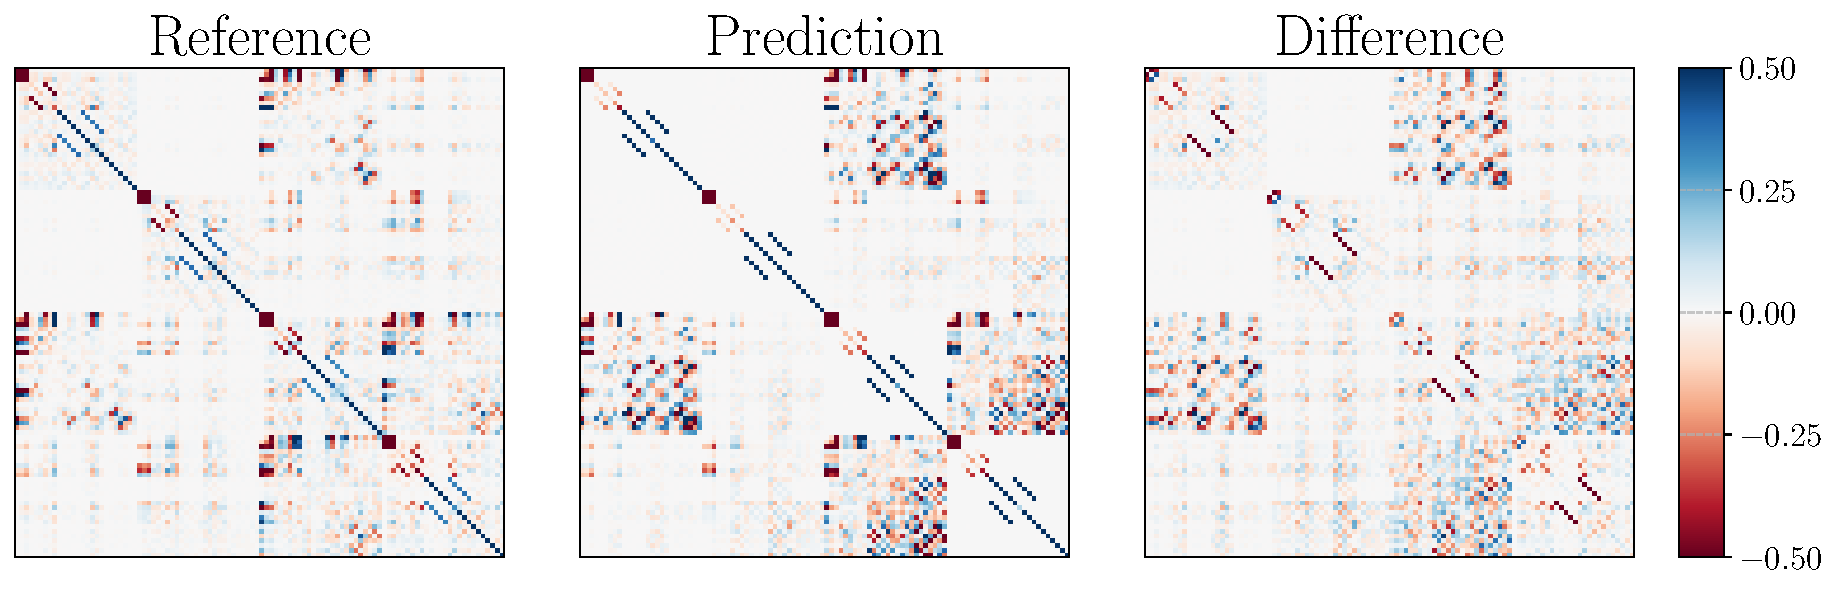
\includegraphics[width=\textwidth]{../fig/mlp_further_trials/fock_truth_vs_pred.pdf}
    \caption[MLP vs. reference Fock]{Reference (fully converged Fock matrix) vs. predicted Fock matrix using the MLP model and the GWH re-construction and element-wise difference for \texttt{dsgdb9nsd\_082452}. Plots only show entries for two \ch{O} (upper left) and two \ch{C} (lower right) atoms and their respective off-diagonal elements.}
    \label{fig:comparison_mlp_gwh_fock}
\end{figure}

\begin{figure}[H]
    \centering
    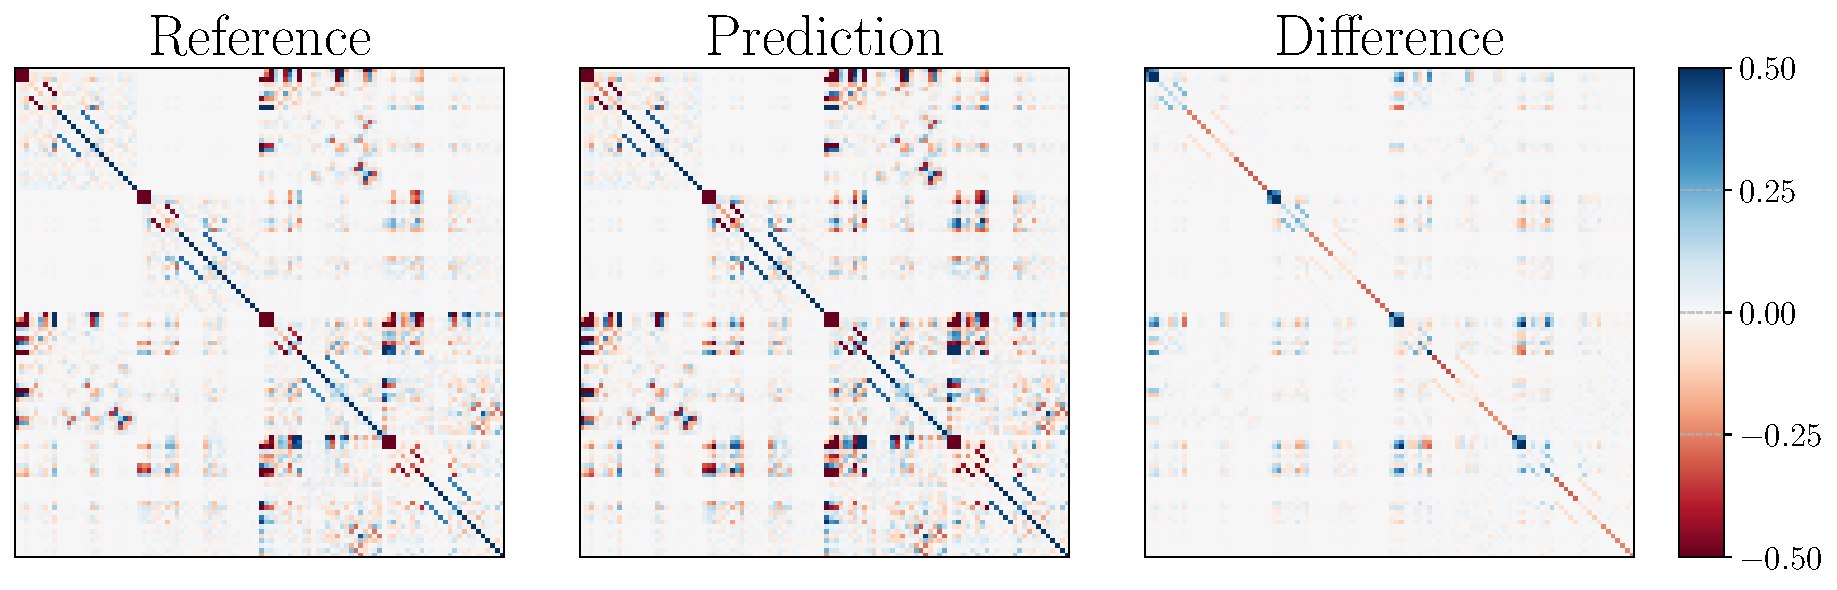
\includegraphics[width=\textwidth]{../fig/mlp_further_trials/fock_truth_vs_minao.pdf}
    \caption[\texttt{minao} vs. reference Fock]{Reference (fully converged Fock matrix) vs. Fock matrix constructed via \texttt{minao} guess and element-wise difference for \texttt{dsgdb9nsd\_082452}. Plots only show entries for two \ch{O} (upper left) and two \ch{C} (lower right) atoms and their respective off-diagonal elements.}
    \label{fig:comparison_minao_fock}
\end{figure}
Comparing \autoref{fig:comparison_mlp_gwh_fock} and \autoref{fig:comparison_minao_fock}, the difference in error patterns is apparent. While the MLP model performs well on the main diagonal, the GWH reconstruction cannot adequately capture the off-diagonal elements, thus resulting in a high RMSE of $0.085$ compared to $0.029$ for the \texttt{minao} guess. Given that many entries are zero—thereby artificially lowering the overall RMSE—the roughly three-fold difference further highlights the substantial underperformance of the GWH reconstruction compared to the \texttt{minao} guess.\\
To get the density from our Fock matrices we solve \autoref{eq:density_reconstruction_from_fock} and gather the lowest $n_{occ}$ eigenvectors to build the coefficients and subsequently the density matrix. \autoref{fig:comparison_mlp_gwh_density} shows the density obtained by this procedure and compares it to the density obtained from the \texttt{minao} guess.

\begin{figure}[H]
    \centering
    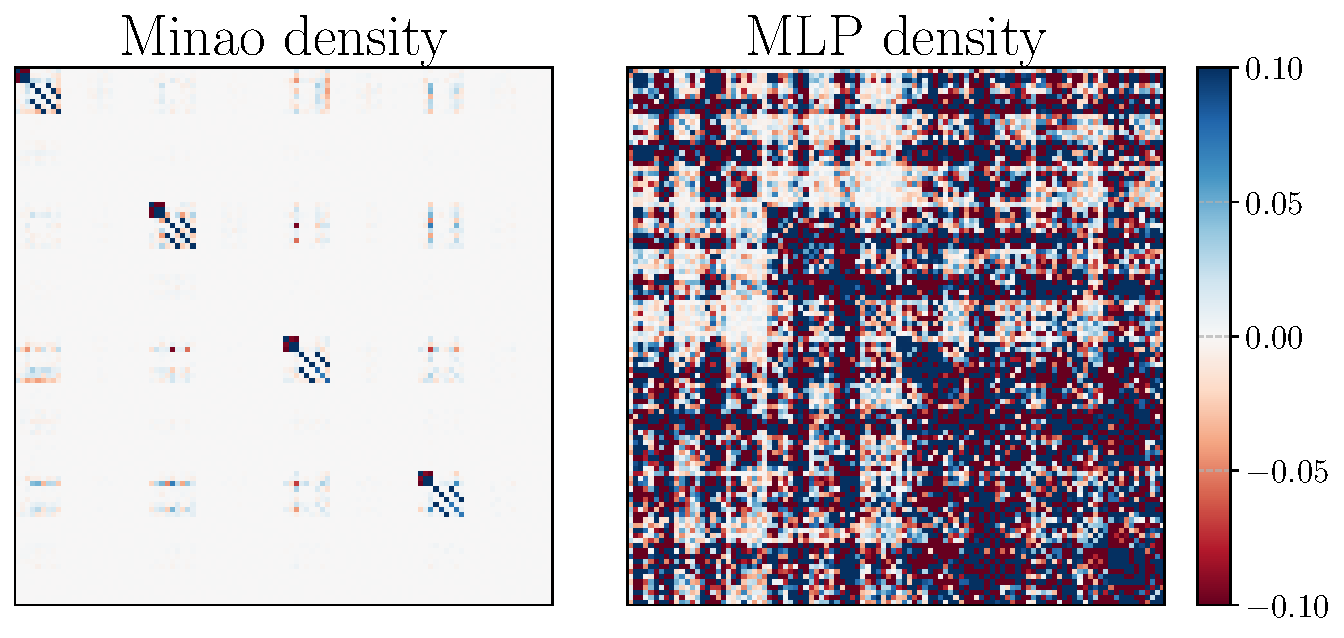
\includegraphics[width=0.7\textwidth]{../fig/mlp_further_trials/minao_vs_pred.pdf}
    \caption[\texttt{minao} vs. MLP density]{\texttt{minao} density vs. density given by the diagonalisation of the Fock prediction from the MLP model for \texttt{dsgdb9nsd\_082452}. Plots only show entries for two \ch{O} (upper left) and two \ch{C} (lower right) atoms and their respective off-diagonal elements.}
    \label{fig:comparison_mlp_gwh_density}
\end{figure}
While \texttt{minao} provides a sparse density matrix, our MLP implementation yields a very dense result with many non-zero-off-diagonal elements. This directly stems from the fact that GWH does introduce large errors in the Fock matrix which propagate through the eigenvalue problem to the density matrix. \\
A qualitative benchmark of the iteration count until convergence offers a similar picture as before: Calculations using the \texttt{minao} guess converge in roughly 11 iterations, while the simulations using the MLP model with GWH reconstruction take around 20 iterations. The present model thus performs similar to other basic initialization schemes such as the \texttt{1e} guess. Interestingly, our model and the \texttt{1e} guess do not offer statistically relevant benefits in terms of iterations compared to a randomly initialized density matrix as seen in \autoref{tab:mlp_metrics}.
\begin{table}[h]
    \centering
    \caption[\ch{C7H10O2} subset - iterations to convergence MLP]{Iterations needed to convergence for different guessing schemes on the \ch{C7H10O2} test subset. MLP\_GWH uses the MLP prediction with GWH reconstruction of Fock off-diagonals and subsequent derivation of density matrix. The \texttt{random} column refers to a random density guess in the range $[-0.5, 0.5]$}
    \label{tab:mlp_metrics}
    \begin{tabular}{l
                    S[table-format=2.1(1)]
                    S[table-format=2(1)]
                    S[table-format=2.1(1.1)]
                    S[table-format=2.1(1.1)]}
        \toprule
        Method          & {minao} &{1e}& {MLP\_GWH}        & {random}  \\
        \midrule
        Iterations (\#) & 10.8(4) & 19(3)  & 19.8(1.0) & 19.8(1.2)       \\
        \bottomrule
    \end{tabular}
\end{table}

\section{Conclusion}
\label{sec:fock_matrix_prediction_conclusion}
This chapter introduced an approach to predict the density matrix by first estimating the Fock matrix and then reconstructing the density via diagonalisation. Initial experiments on the \ch{C5H4N2O2} subset of QM9 showed that linear models (Ridge Regression and Kernel Ridge Regression) can learn the Fock matrix reasonably well but fail to match the accuracy of established PySCF guessing schemes such as \texttt{minao} and \texttt{vsap} in terms of iterations until convergence. When scaling up to a larger 6-31G(2df,p) basis and the \ch{C7H10O2} isomer set, a single-layer MLP captured the Fock diagonal with low RMSE, yet the generalized Wolfsberg-Helmholtz reconstruction of off-diagonals introduced large errors. Diagonalisation amplifies these errors, producing a noisy density matrix and nearly doubling SCF iterations ($\approx20$ vs. 11).

Overall, while the ML-based Fock prediction pipeline can outperform simple Hückel or one-electron guesses in diagonal accuracy, it still underperforms in convergence speed and off-diagonal fidelity compared to better physics-based schemes. This suggests that a one-shot prediction of the full Fock matrix simultaneously ans subsequent density derivation is infeasible. Accounting for local interactions and directly predicting a sparse density matrix (compared to the Fock matrix) may perform  better. We shall explore the latter approach in the next chapter by representing the molecular structure using a Graph Neural Network (GNN). 


\chapter{A GNN approach to the problem}
\label{chap:gnn}

\TODO{
    \begin{itemize}
        \item Design - Blocks and Subblocks \& abstraction
        \item Data prep - Data augmentation (Wigner D-Matrices etc. )
        \item GNN Design
        \item GNN Training + Benchmarking 
    \end{itemize}
}

\section{Input \& Output Matrices}
\label{sec:gnn_input_output_matrices}
\section{Data Augmentation}
\label{subsec:gnn_data_augmentation}
Our input (overlap) as well as our output (Fock matrix) are quantities which are not generally invariant under rotations of our molecular system. In essence this means that we must find a way to learn differently rotated molecules and produce their respective Fock matrices to later deduce our initial density. While initially the idea of making the input invariant under rotation by using a predetermined standard orientation to learn the problem was considered, problems arise with this approach. Most prominently, defining a standard orientation for isomers / isomer-parts (such as \ch{C7H10O2} or submolecules thereof) is far from trivial. Even if such a standard orientation is defined, one has to consider an additional pre- and post-processing step to rotate the input into the standard orientation and the output back to the original orientation. \\
Contrary to this, the model can learn differently rotated inputs to generate the corresponding outputs. This is achieved by augmenting the dataset with different rotations of the same molecules / submolecules. Rotating the input coordinates using a rotation matrix $R$ is in principle rather straightforward. However, the corresponding overlap, density and Fock matrices also have to be transformed accordingly or recalculated. The later is computationally not feasible, hence we use the corresponding Wigner D-matrices to transform input and output matrices. 
The Wigner D-matrix is a unitary matrix with $2L + 1$ rows and columns, where $L$ is the angular momentum. For a given rotation $R$ the Matrix elements of overlap, density and Fock matrix transform as follows:
\begin{equation}
    O'_{ij} = \sum_{k,l} \mathcal{D}^{(L)}_{ik}(R) O_{kl} \mathcal{D}^{(L)*}_{lj}(R)
\end{equation}
Naturally the transformation only acts on spatial orbitals with no rotational symmetry along the axis of rotation (i.e. $L \neq 0$). Given our blocks defined in \autoref{sec:gnn_input_output_matrices} $\mathcal{D}^{(L)}$ will only transform hetero-blocks with at least one orbital having $L \neq 0$. \\

\TODO{Idea next paragraph: }
Practically, the data is augmented by sampling a random rotation axis (TODO: constraints of this axis) and a random rotation angle $\theta \in [0, 2\pi]$. Given this axis and angle, the corresponding transformations are performed to the overlap, density and Fock matrices to obtain our augmented samples. 
Due to the grid spacing in DFT calculations small deviations ($\approx 0,1 \unit{\milli\hartree}$) between the transformed matrices and newley calculated ones occur.
%! Note that translating the molecule should change absolutely nothing about the Overlap or Fock matrix. 

\section{GNN Design}
\label{sec:gnn_design}

\section{Training}
\label{sec:gnn_training}
\TODO{better text}
We initially train a model without data augmentation and only on a small subset of our QM9 C7H10O2 molecules (500 atoms simulated with B3LYPG \& pcseg-1) with a 80/10/10 split (train/val/test). 
Meta: 
\begin{verbatim}
batch_size=16,
hidden_dim=256,
train_val_test_ratio=(0.8, 0.1, 0.1),
message_passing_steps=3,
edge_threshold_val=5,
message_net_layers=3,
message_net_dropout=0.1,
target="fock",
lr=1e-3 
weight_decay=1e-5
trained for 103 epochs (overfitting started earlier - 
see history data in scripts>gnn>plot_data)
test_loss: 6.00
using standards from c2ec04be68ae09bec80153fabaace85234ad1a5e elsewhere!
\end{verbatim}
        
\begin{figure}[H]
    \centering
    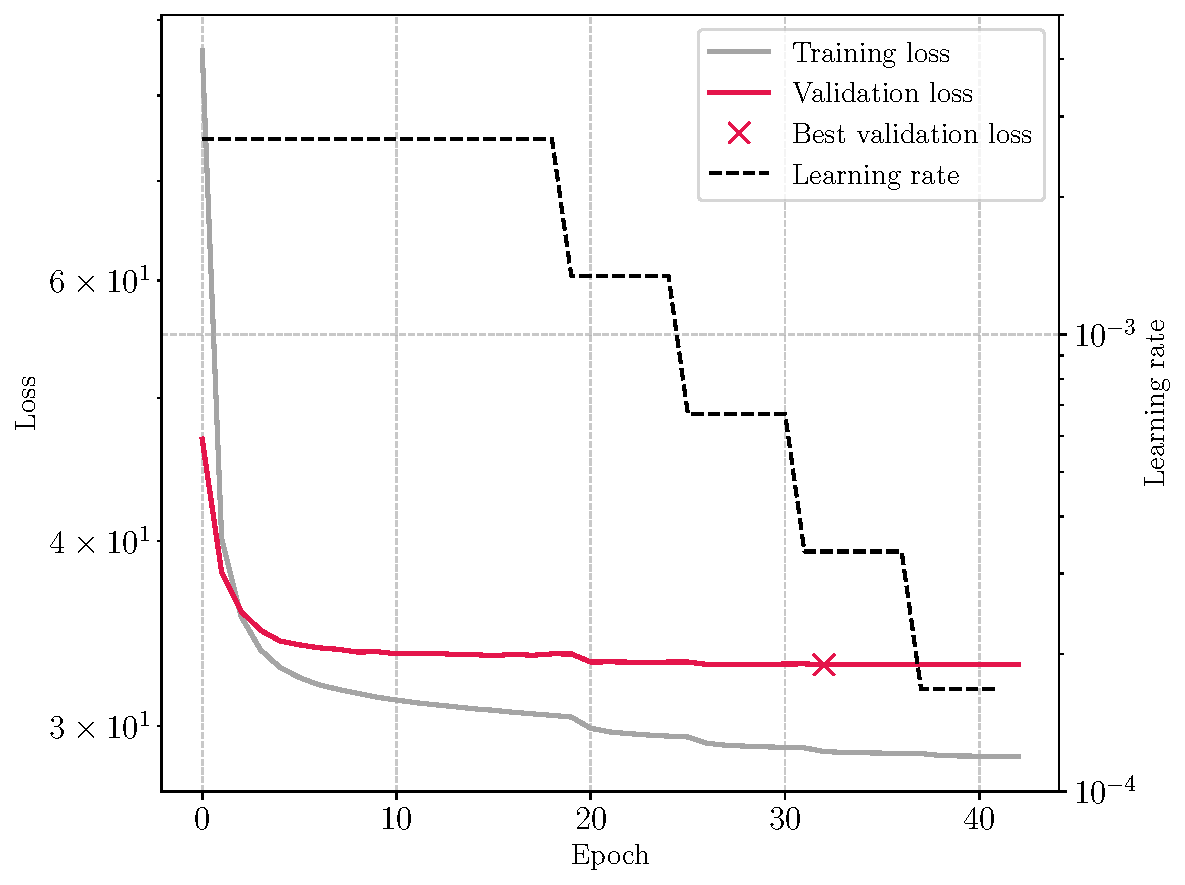
\includegraphics[width=\textwidth]{../fig/gnn/mgnn_pcseg1_simple_loss.pdf}
    \caption[GNN initial training Loss]{\TODO{...}}
    \label{fig:gnn_initial_training_loss}
\end{figure}
\chapter{Application}
\label{chap:application}
The GNN model introduced in \autoref{chap:gnn} will be benchmarked on various datasets in the following sections. All reference data was calculated using the 6-31G(2df,p) basis at theory level B3LYP. 

Models will be evaluated by their iteration count until convergence, by the energy difference from the converged solution the DIIS error (see \autoref{eq:diis_error}), and by the RMSE. The inference time of all models, just a few milliseconds, is roughly three orders of magnitude shorter than that of a typical DFT calculation, and can therefore be regarded as negligible. This performance holds across all applications discussed below.

\section{QM9 - \ch{C7H10O2} Isomers}
\label{sec:qm9_isomers_benchmark}
There are 6095 structural isomers of \ch{C7H10O2} in the QM9 dataset (see \autoref{sec:dataset}). Analogous to the trials performed in \autoref{sec:further_trials_mlp}, we will train and validate on a randomly drawn sample of 500 isomers\footnote{using \textsc{scf\_guess\_datasets} (see \autoref{subsec:gnn_normalization})}. This reduction is necessary to make training and hyperparameter-tuning feasible in the scope of the thesis. Contrary to the full matrix prediction schemes of \autoref{chap:fock_matrix_predictions}, we employ sub-matrix predictions and reconstruct the full matrix, thus increasing the actual number of samples significantly. Per molecule, we obtain 7, 10 and 2 samples for \ch{C}, \ch{H} and \ch{O}, respectively, yielding a total of 3500 \ch{C}, 5000 \ch{H} and 1000 \ch{O} samples. This already provides a certain rotational variability, but additional rotations can be introduced through data augmentation during training to develop a model that is insensitive to rotation when predicting density.
\newpage
\subsection{Initial training}
\label{subsec:qm9_isomers_initial}
%! refer to MGNN_6-31G_NO_AUG_07_07_manual_ref.pth
To evaluate the performance of the GNN devised in \autoref{chap:gnn}, several manual runs were initiated during development, with hyperparameters set to the values listed in \autoref{tab:init_hparams}. 
\begin{table}[H]
    \centering
    \caption[Hyperparameters - initial MGNN training (manually selected)]{Hyperparameters used for the initial MGNN training (manually selected)}
    \label{tab:init_hparams}
    \begin{tabular}{ll ll}
        \toprule
        \textbf{Hyperparameter} & \textbf{Value} & \textbf{Hyperparameter} & \textbf{Value} \\
        \midrule
        Hidden dimension & 256 & Msg. passing rounds & 4 \\
        MsgNet layers & 3 & MsgNet dropout & 15 \% \\
        Batch size & 16 & Grace period & 10 epochs \\
        Target & Density matrix & Loss function & MSE (blockwise) \\
        Learn rate (initial) & $2.68 \times 10^{-3}$ & Weight decay & $1.78 \times 10^{-5}$ \\
        Edge threshold & 3 \AA & Data augmentation & No \\
        \midrule
        Learn rate factor & 0.5 & Learn rate patience & 3 epochs \\
        Learn rate threshold & $10^{-3}$ & Learn rate cooldown & 2 epochs \\
        Learn rate min & $10^{-6}$ & — & — \\
        \bottomrule
    \end{tabular}
\end{table}
Note that these initial runs did not use data augmentation, so the training comprised 400 samples (80\% of our data), leaving 10\% for validation and 10\% for testing. The grace period (time without improvement) was set to 10 epochs to leave the learning rate scheduler sufficient time to take effect.\\

Training and validation losses both monotonically decrease until around epoch 30. As can be seen in \autoref{fig:initial_train_qm9_isomers}, while the loss on the validation set flattens out rather early, training loss decreases throughout the entire training process. 
\begin{figure}[H]
    \centering
    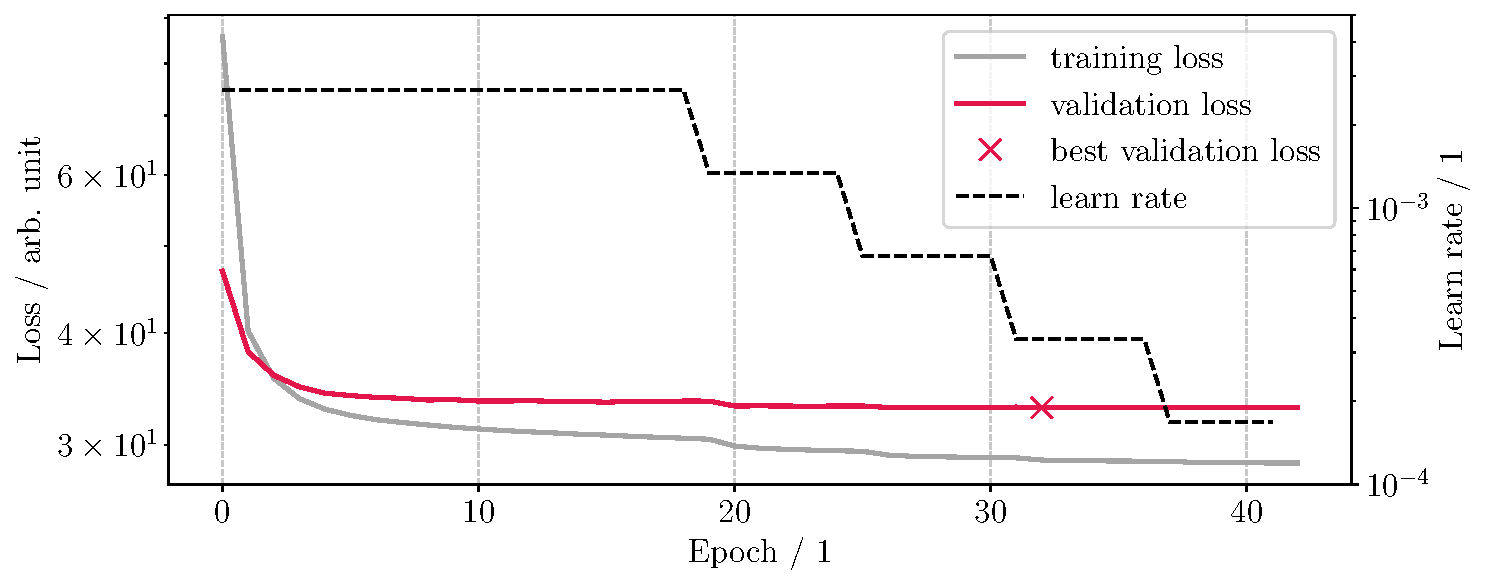
\includegraphics[width=0.75\textwidth]{../fig/gnn/MGNN_6-31G_NO_AUG_07_07_manual_ref_train_val_loss.pdf}
    \caption[Initial GNN loss on QM9-isomers]{Initial GNN training/ validation loss and corresponding learn rate per epoch on QM9-isomers.}
    \label{fig:initial_train_qm9_isomers}
\end{figure}
Both losses are reduced further by stepwise decrease of the learn rate. This run produced the best model in epoch 33, with a validation loss of $33.00$ and a training loss of $28.83$, indicating slight overfitting which is to be expected especially without data augmentation in the training samples. The performance of the model $\text{GNN}_\text{initial}$ on the test set is compared to other models and the various guessing schemes in a summarizing \autoref{tab:qm9_isomers_test_overview} placed at the end of this chapter. 

\subsection{Hyperparameter tuning}
\label{subsec:qm9_isomers_hyperparamtuning}
Validation loss is used as a benchmark to select the best model from a hyperparameter run. While we will also prefer models with lower loss, we must be very careful not to select models which look good on paper but perform worse due to the lack of sufficient correlation between MSE and iteration count. For this reason, we will base our hyperparameter search on the $\text{GNN}_\text{initial}$ model and explore the hyperparameter space in a structured way. 

\textbf{Data augmentation}\\
$\text{GNN}_\text{initial}$ already performed quite well in terms of iterations without using any data augmentation. One might argue that there is already some data augmentation intrinsic to the training set due to the different orientations of atoms in various molecules. 
\begin{figure}[H]
    \centering
    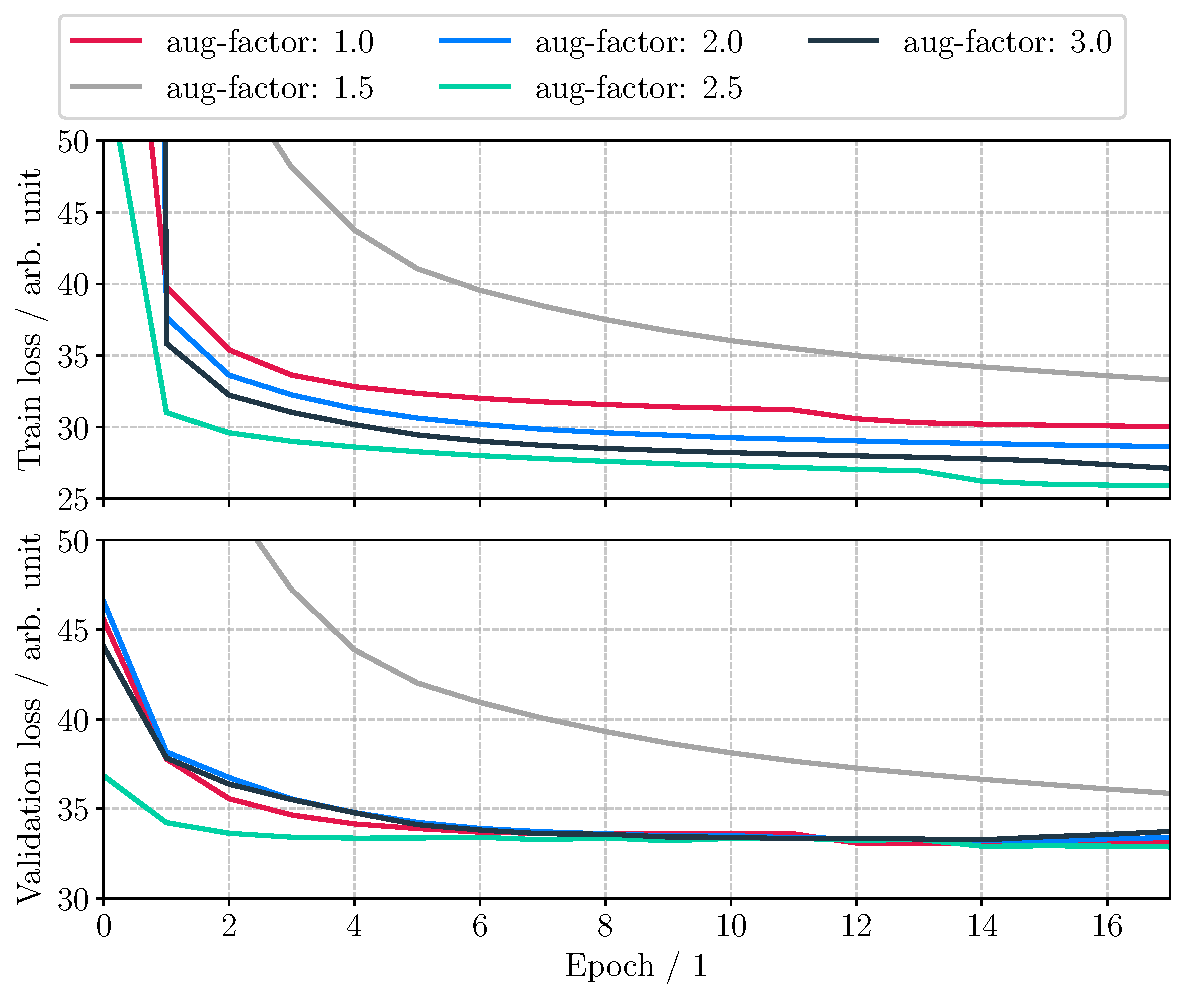
\includegraphics[width=0.75\textwidth]{../fig/application/aug_train_val_loss.pdf}
    \caption[GNN loss for different augmentation factors on QM9-isomers]{GNN loss for different data augmentation factors on QM9-isomers. All other hyperparameters are chosen as in \autoref{tab:init_hparams}.}
    \label{fig:loss_hyper_qm9_isomers}
\end{figure}
A comparison of the training and validation loss between different augmentation factors in \autoref{fig:loss_hyper_qm9_isomers} shows no clear trend regarding the choice of the augmentation factor. While a factor of $2.5$ initially outperforms no augmentation and other factors, they all converge in validation eventually. 
Investigating different metrics on the test set in \autoref{tab:qm9_isomers_data_aug_hyperparam} does not yield a conclusive insight. Our initial model has the best performance in terms of iterations; however, other models do not fall far behind in this metric. Furthermore, no statistically significant correlation was found between the number of iterations and other metrics, including the energy errors ($|\Delta E_\text{DFT}|$ and relative $|\delta E_\text{DFT}|$), the DIIS error, and the RMSE.
\begin{table}[H]
    \centering
    \caption[GNN on QM9 isomers with different data augmentation factors]{GNN performance on the QM9 \ch{C7H10O2} isomers test set for different data augmentation factors\footnotemark. For each factor, the table lists the mean and standard deviation of the following metrics: iterations until convergence, $|\Delta E_\text{DFT}|$ (absolute energy difference to the reference DFT calculation), $|\delta E_\text{DFT}|$ (relative energy difference to the reference DFT calculation), DIIS error (as defined in \autoref{eq:diis_error}), and root mean square error (RMSE) between the predicted and converged density matrices. Energies are given in Hartree ($\unit{\hartree}$).}
    \label{tab:qm9_isomers_data_aug_hyperparam}
    \resizebox{\textwidth}{!}{
        \begin{tabular}{S[table-format=1.1]
                        S[table-format=2.1(1.1)]
                        S[table-format=-1.1(1.1)]
                        S[table-format=-1.4(1.1)]
                        S[table-format=1.3(1)]
                        S[table-format=1.4(1)]}
            \toprule
            {Augmentation factor / 1} & {Iterations / 1} & {$|\Delta E_\text{DFT}|$ / $\unit{\hartree}$}  & {$|\delta E_\text{DFT}|$ / 1} & {DIIS error / $\unit{\hartree}$} & {RMSE / 1} \\
            \midrule
            1.0 & \B 11.2(6)  & \B 0(3) & \B 0.0000(16)  & 0.027(0.004) & \B 0.0078(6) \\
            1.5 & 11.3(6)           & 1.4(17) & 0.0008(10)          & 0.027(0.004) & 0.0079(6)\\
            2.0 & 11.5(6)           & \B 0(3) & 0.0001(14)     & \B 0.027(3)  & 0.0079(6)\\
            2.5 & 12.0(7)           & 1(4)   & 0.001(2)            & 0.029(0.003) & 0.0080(6)\\
            3.0 & 11.4(8)           & 1(3)   & 0.0006(18)          & 0.031(0.007) & 0.0081(6)\\
            3.5 & 11.3(6)           & 2(3)   & 0.0013(18)          & 0.029(0.003) & 0.0080(6)\\
            4.0 & 11.6(10)          & 2(4)    & 0.001(3)            & 0.029(0.003) & 0.0080(6)\\
            \bottomrule
        \end{tabular}
        }
\end{table}
\footnotetext{Other hyperparameters are set according to \autoref{tab:init_hparams}.}
\textbf{Investigating Edge Threshold Distance}\\
The edge threshold distance has an immediate impact on message passing between nodes. It essentially acts as a cutoff that determines whether an edge between two nodes is formed. Keeping it rather short, in the vicinity of bond-lengths will only connect directly bound neighbours. On the other hand, a higher threshold distance allows the formation of longer ranging connections in the GNN. \autoref{tab:qm9_isomers_dist_hyperparam} shows the influence on the metrics for varying threshold distances.  
\begin{table}[H]
    \centering
    \caption[GNN on QM9 isomers with different edge threshold distances]{GNN performance on QM9 \ch{C7H10O2} isomers test set for different edge threshold distances (given in $\unit{\angstrom}$). Other hyperparameters are set according to \autoref{tab:init_hparams}.}
    \label{tab:qm9_isomers_dist_hyperparam}
    \resizebox{\textwidth}{!}{
        \begin{tabular}{S[table-format=1.1]
                        S[table-format=2.1(1.1)]
                        S[table-format=-4(2)]
                        S[table-format=-1.3(2)]
                        S[table-format=1.3(1.1)]
                        S[table-format=1.4(1)]}
                        \toprule
                        {Threshold distance / $\unit{\angstrom}$} & {Iterations / 1} & {$|\Delta E_\text{DFT}|$ / $\unit{\hartree}$}  & {$|\delta E_\text{DFT}|$ / 1} & {DIIS error / $\unit{\hartree}$} & {RMSE / 1} \\
                        \midrule
                        1.5 & 15.1(19)& 1(13)        & 0.001(0.008)   & 0.045(0.005) & 0.0104(5)\\
                        2.0 & 12.3(9) & 4.1(0.8)     & 0.0024(0.0005) & 0.034(0.005) & 0.0084(5)\\
                        2.5 & \B 11.2(6) & 1(2)& 0.0006(0.0012) & 0.026(0.004) & 0.0081(6)\\
                        3.0 & 11.8(13)& 1(6)         & 0.001(0.003)   & 0.027(0.003) & 0.0079(6)\\
                        3.5 & 12.6(8) & 1(2)         & 0.0010(0.0011) & \B 0.025(4) & 0.0077(6)\\
                        4.0 & 12.0(9) & 2(4)         & 0.001(0.002)   & \B 0.025(4) & 0.0078(6)\\
                        4.5 & 12.4(10)& \B 0(7)& \B 0.000(4)& 0.027(0.004) & 0.0080(6)\\
                        5.0 & 11.2(7) & 1(2)         & 0.0005(0.0012) & \B 0.025(4) & \B 0.0077(7)\\
            \bottomrule
        \end{tabular}
    }
\end{table}
For a low distance threshold of $\SI{1.5}{\angstrom}$, which lies around the bond length of \ch{C}-\ch{C} bonds, worse performance in terms of iterations is attained compared to higher threshold distances. 

\textbf{Further hyperparameter optimization runs}\\
For all training runs up until now, the training loss was evaluated only on the normalized sub matrices included in training. In practice, this means that the network has generally lower loss for low cutoff distances because fewer interaction blocks are included in the loss calculation. In the next step, we investigate whether changing the loss to a full matrix loss will impact GNN prediction performance. \autoref{tab:qm9_isomers_further_runs} shows ten different configurations evaluated on the test set. 
\begin{table}[H]
    \centering
    \caption[GNN on QM9 isomers training with full matrix loss]{GNN on QM9 isomers using full matrix loss and a maximum of 30 epochs to train. Metrics on test set and corresponding hyperparameter settings for the five best performing networks (0-4) from search and five sampled ones (5-9) from same hyperparameter search.}
    \label{tab:qm9_isomers_further_runs}
    \resizebox{\textwidth}{!}{
        \begin{tabular}{l
                        S[table-format=2.1(1.1)]
                        S[table-format=-4(2)]
                        S[table-format=-1.3(2)]
                        S[table-format=1.3(1)]
                        S[table-format=1.4(1)]}
            \toprule %!rerun DONE
            Models                 & {Iterations / 1} & {$|\Delta E_\text{DFT}|$ / $\unit{\hartree}$}  & {$|\delta E_\text{DFT}|$ / 1} & {DIIS error / $\unit{\hartree}$} & {RMSE / 1} \\
            \midrule
            $\text{GNN}_\text{f. 0}$ & \B 11.5(9) & 0.7(14)    & 0.0004(8) & 0.028(4) & \B 0.0076(6) \\ %41
            $\text{GNN}_\text{f. 1}$ & 11.6(0.7)        & \B 0.2(17)& \B 0.0001(10)& \B 0.027(4) & 0.0078(0.0006) \\ %73
            $\text{GNN}_\text{f. 2}$ & 11.7(0.8)        & 18.0(18)   & 0.0103(10)& 0.029(3) & 0.0079(0.0006) \\%57
            $\text{GNN}_\text{f. 3}$ & 13.1(1.1)        & 0.3(14)    & 0.0002(8) & 0.035(5) & 0.0084(0.0005) \\ %12
            $\text{GNN}_\text{f. 4}$ & 13.2(1.1)        & 2.3(10)    & 0.0013(6) & 0.040(6) & 0.0088(0.0005) \\ %144
            $\text{GNN}_\text{f. 5}$ & 13.3(1.1)        & 2(3)       & 0.0014(15)& 0.042(4) & 0.0090(0.0005) \\ %95
            $\text{GNN}_\text{f. 6}$ & 13.6(1.0)        & 1(2)       & 0.0004(13)& 0.042(2) & 0.0089(0.0005) \\ %82
            $\text{GNN}_\text{f. 7}$ & 13.9(1.1)        & 1.5(16)    & 0.0008(9) & 0.041(3) & 0.0088(0.0006) \\ %9
            $\text{GNN}_\text{f. 8}$ & 14.5(1.4)        & 0.9(7)     & 0.0005(4) & 0.040(2) & 0.0090(0.0005) \\ %79
            $\text{GNN}_\text{f. 9}$ & 14.7(1.2)        & 7(3)       & 0.0043(18)& 0.042(3) & 0.0091(0.0005) \\ %70
            \bottomrule
        \end{tabular}
    }
        \resizebox{\textwidth}{!}{
        \begin{tabular}{lrrrrrrrrrr}
        \toprule
        Parameters & $\text{GNN}_\text{f. 0}$ & $\text{GNN}_\text{f. 1}$ & $\text{GNN}_\text{f. 2}$ & $\text{GNN}_\text{f. 3}$ & $\text{GNN}_\text{f. 4}$ & $\text{GNN}_\text{f. 5}$ & $\text{GNN}_\text{f. 6}$ & $\text{GNN}_\text{f. 7}$ & $\text{GNN}_\text{f. 8}$ & $\text{GNN}_\text{f. 9}$ \\
        \midrule
        Hidden dimension & 512 & 256 & 128 & 128 & 128 & 512 & 256 & 128 & 256 & 256 \\
        Batch size & 8 & 8 & 8 & 8 & 32 & 32 & 32 & 32 & 32 & 32 \\
        Data aug. factor & 1.83 & 2.46 & 2.38 & 1.76 & 1.50 & 1.14 & 1.67 & 2.45 & 1.91 & 2.33 \\
        Edge threshold & 2.73 & 3.87 & 3.21 & 2.07 & 2.11 & 2.11 & 2.14 & 2.12 & 2.11 & 2.05 \\
        Message passing steps & 2 & 4 & 3 & 3 & 4 & 2 & 3 & 2 & 3 & 3 \\
        Message Net dropout & 0.10 & 0.27 & 0.21 & 0.18 & 0.29 & 0.14 & 0.18 & 0.23 & 0.22 & 0.11 \\
        Message Net layers & 3 & 5 & 4 & 3 & 5 & 3 & 3 & 3 & 5 & 3 \\
        Learn rate & 6.34e-04 & 2.31e-04 & 2.89e-04 & 4.93e-03 & 3.97e-03 & 1.79e-04 & 3.54e-04 & 4.36e-03 & 2.61e-04 & 1.16e-04 \\
        Weight decay & 4.56e-04 & 7.37e-05 & 4.37e-05 & 1.69e-05 & 9.97e-04 & 8.35e-05 & 5.21e-05 & 4.43e-05 & 2.97e-04 & 2.35e-05 \\
        \bottomrule
        \end{tabular}
        }
\end{table}
The best performing networks using full matrix loss perform slightly worse with regard to iteration count. Notably, $\text{GNN}_\text{f. 0}$ reaches the lowest RMSE of all benchmarked models so far. Correlation between our surrogate metrics and iterations is rather high for DIIS and RMSE, with a Pearson correlation coefficient of $0.91$ and $0.94$ respectively. 
Contrary, there is no correlation between the energy errors $|\Delta E_\text{DFT}|$ and $|\delta E_\text{DFT}|$ and the number of iterations. When interpreting these correlations, caution is necessary because they only hold under the specific conditions (GNN trained using full matrix loss) in which they were measured. Bellow, we will see that these relationships exhibit limited generalizability across different guessing schemes.
\newpage
\subsection{Evaluation \& Conclusion}
\label{subsec:qm9_isomers_eval_and_concl}
The top performing models as defined above are now compared to \textsc{PySCF} guessing schemes. A summary of this comparison is provided in \autoref{tab:qm9_isomers_test_overview}.
\begin{table}[H]
    \centering
    \caption[Models compared to \textsc{PySCF} and $\overline{P}$ schemes - \ch{C7H10O2} Isomers]{Comparison of different models with \textsc{PySCF} and $\overline{P}$ guessing schemes for QM9 - \ch{C7H10O2} Isomers.}
    \label{tab:qm9_isomers_test_overview}
    \resizebox{\textwidth}{!}{
        \begin{tabular}{l
                        S[table-format=2.1(1.1)]
                        S[table-format=-4(3)]
                        S[table-format=-1.3(2)]
                        S[table-format=1.4(1.1)]
                        S[table-format=1.4(1)]}
            \toprule
            Guessing schemes                 & {Iterations / 1} & {$|\Delta E_\text{DFT}|$ / $\unit{\hartree}$}  & {$|\delta E_\text{DFT}|$ / 1} & {DIIS error / $\unit{\hartree}$} & {RMSE / 1} \\
            \midrule
            $\text{GNN}_\text{initial}$   &11.2(6)   & \B 0(3)& \B 0.0000(16) & 0.027(0.004) & 0.0078(6)\\ %initial
            $\text{GNN}_\text{f. 0}$      & 11.5(9)  & 0.7(14)    & 0.0004(8) & 0.028(4) & \B 0.0076(6) \\ %41
            $\overline{P}$                & 17.1(15) & 211(6)      & 0.1208(19)& 0.110(3)  & 0.0137(4)\\
            \texttt{1-e}                  & 18.8(18) & 220(30)     & 0.128(19) & 0.1220(10)& 0.14(4)  \\
            \texttt{vsap}                 & 14.2(9)  & 5.4(4)      & 0.0030(2) & \B 0.026(2) & 0.0109(7)\\
            \texttt{atom}                 & 16.6(19) & 14(4)       & 0.007(3)  & 0.044(7) & 0.016(2) \\
            \texttt{minao}                & \B 10.8(6)& 2.8(2)&0.00162(12)& 0.077(3) & 0.0155(4)\\
            \bottomrule
        \end{tabular}
    }
\end{table}
A direct comparison of \textsc{PySCF} and $\overline{P}$ guessing schemes with our GNN approach already offers several insights. Examining the relationship between energy errors and the number of iterations shows that guesses with smaller energy errors ($|\Delta E_\text{DFT}|$) tend to convergence faster. 
Furthermore, a low DIIS alone will not necessarily translate into fast convergence of the guessed density. The GNN approach surpasses most conventional guessing schemes and performs nearly on par with \texttt{minao} in terms of iterations. Varying the data augmentation factor had negligible effect on the convergence speed, while the distance threshold contributes for distances around the bond length. However, it remains to be seen how well these models generalize to other data. 

\section{QM9 - \ch{C7H10O2} Molecular Dynamics (MD)}
\label{sec:qm9_md_isomers_benchmark}
So far, all predictions have considered only ground state geometries. While predicted and calculated traits of the ground state give invaluable insight into the chemical properties, the behaviour of the molecules in more attainable environments is of interest. The MD trajectories of \ch{C7H10O2} dataset \parencite{ref:qm9_isomers_md} constitute a randomly sampled set of 113 isomers from the QM9 \ch{C7H10O2} data. The trajectory of every isomer is calculated every $\SI{1}{\femto\second}$ for 5000 steps at a temperature of 500 K using the PBE exchange-correlation potential (see \ref{subsec:background_dft}). From these geometries, 500 are sampled to calculate a reference data set using the 6-31G(2df,p) basis at the B3LYP level of theory. This combination is employed in all following computer experiments. 
\newpage
\subsection{Zero-shot predictions}
\label{sec:qm9_md_isomers_zero_shot}
Zero-shot predictions are made on inputs outside the training set's scope. In our case, a model previously trained on the QM9 \ch{C7H10O2} isomer set may be used to predict the density for a given MD sample. Prediction metrics using the pre-trained models from \autoref{sec:qm9_isomers_benchmark} on the MD test set are given in \autoref{tab:qm9_md_zero_shot}. 
\begin{table}[H]
    \centering
    \caption[GNN zero-shot predictions on QM9 \ch{C7H10O2} isomer MD]{GNN zero-shot predictions on the QM9 \ch{C7H10O2} isomer MD test set. $\text{GNN}_\text{initial}$ and $\text{GNN}_\text{f. 0}$ were trained using the QM9 \ch{C7H10O2} isomer set.}
    \label{tab:qm9_md_zero_shot}
    % \resizebox{\textwidth}{!}{
        \begin{tabular}{l
                        S[table-format=2.1(1)]
                        S[table-format=-4(2)]
                        S[table-format=-1.3(1.1)]
                        S[table-format=1.2(1.1)]
                        S[table-format=1.4(1.1)]}
            \toprule
            Models                 & {Iterations / 1} & {$|\Delta E_\text{DFT}|$ / $\unit{\hartree}$}  & {$|\delta E_\text{DFT}|$ / 1} & {DIIS error / $\unit{\hartree}$} & {RMSE / 1} \\
            \midrule
            $\text{GNN}_\text{initial}$   & 11.4(9)    & 1(2)     & 0.0007(11)  & 0.026(3)& 0.0079(4) \\ %!- do full rerun + iterations with model from data_aug_1.0 -> done and already updated
            $\text{GNN}_\text{f. 0}$      & 11.3(8)  & 1.3(1.1) & 0.0007(6)     & 0.029(3)& 0.0077(4) \\
            \bottomrule
        \end{tabular}
    % }
\end{table}
Both models perform surprisingly well on the unseen data. $\text{GNN}_\text{f. 0}$ even performs slightly better, indicating a generalization to various perturbations of the geometry. Furthermore, $\text{GNN}_\text{initial}$ performs slightly worse on the MD dataset.

\subsection{Hyperparameter tuning}
\label{sec:qm9_md_isomers_hyp_tuning}
%! full matrix run in tune_logs_MGNN_hyp_small_full_mat_loss_md
Metrics for re-trained versions of $\text{GNN}_\text{initial}$ and $\text{GNN}_\text{f. 0}$ from \autoref{sec:qm9_isomers_benchmark} are shown in \autoref{tab:qm9_md_last_best_retrain}. While training $\text{GNN}_\text{f. 0}$ on the MD dataset leads to improvements in all metrics, the re-trained version of $\text{GNN}_\text{initial}$ performs worse than the original model on the MD test set.  
\begin{table}[H]
    \centering
    \caption[GNN predictions on QM9 \ch{C7H10O2} isomer MD]{GNN predictions on the QM9 \ch{C7H10O2} isomer MD test set. With MD-re-trained\footnote{models marked with a $*$ are architectures from another dataset re-trained on the current one} versions of $\text{GNN}_\text{initial}$ and $\text{GNN}_\text{f. 0}$.}
    \label{tab:qm9_md_last_best_retrain}
    % \resizebox{\textwidth}{!}{
        \begin{tabular}{l
                        S[table-format=2.1(1.1)]
                        S[table-format=-4(2)]
                        S[table-format=-1.3(2)]
                        S[table-format=1.3(2)]
                        S[table-format=1.4(1)]}
            \toprule
            Models                 & {Iterations / 1} & {$|\Delta E_\text{DFT}|$ / $\unit{\hartree}$}  & {$|\delta E_\text{DFT}|$ / 1} & {DIIS error / $\unit{\hartree}$} & {RMSE / 1} \\
            \midrule
            $\text{GNN}^{\text{MD*}}_\text{initial}$   & 12.3(10)  & 1(4) & 0.001(2)      & 0.035(4)& 0.0086(6) \\ %! comp_models initial - rerun! 
            $\text{GNN}^{\text{MD*}}_\text{f. 0}$      & 11.1(5)  & 0.0(1.0) & 0.0000(6)  & 0.028(3)& 0.0073(5) \\ % comp_models f0
            \bottomrule
        \end{tabular}
    % }
\end{table}
Analogous to the hyperparameter optimization in \autoref{tab:qm9_isomers_further_runs}, we also use full matrix loss for hyperparameter tuning of the specialized MD models in \autoref{tab:qm9_md_further_runs}. Comparing \autoref{tab:qm9_isomers_further_runs} and \autoref{tab:qm9_md_further_runs}, heavier regularization is generally observed in the MD models. Higher data augmentation and a slightly stronger weight decay help with fitting the varied density given by the perturbed geometries. Furthermore, four out of the top five networks have a batch size of eight, introducing more noise and thus regularization into the update steps. \\
\begin{table}[H]
    \centering
    \caption[GNN on QM9 isomers MD training with full matrix loss]{GNN on QM9 isomers MD using full matrix loss and a maximum of 30 epochs to train. Metrics on test set and corresponding hyperparameter settings for the ten best performing networks in terms of iterations.}
    \label{tab:qm9_md_further_runs} %!TODO rerun with all models if there is time!
    \resizebox{\textwidth}{!}{
        \begin{tabular}{l
                        S[table-format=2.1(2)]
                        S[table-format=-4(2)]
                        S[table-format=-1.3(2)]
                        S[table-format=1.3(1)]
                        S[table-format=1.4(1)]}
            \toprule
            Models                 & {Iterations / 1} & {$|\Delta E_\text{DFT}|$ / $\unit{\hartree}$}  & {$|\delta E_\text{DFT}|$ / 1} & {DIIS error / $\unit{\hartree}$} & {RMSE / 1} \\
            \midrule
            $\text{GNN}^{\text{MD}}_\text{f. 0}$ & \B 10.9(5) &  1.5(1.7) & 0.001(0.001) & \B 0.027(3) & \B 0.0075(4) \\
            $\text{GNN}^{\text{MD}}_\text{f. 1}$ & 11.0(4) &   1.8(1.3)  & 0.001(0.001) & 0.030(0.003) & 0.0076(0.0004) \\
            $\text{GNN}^{\text{MD}}_\text{f. 2}$ & 11.2(6) &   3.1(2.2)  & 0.002(0.001) & 0.031(0.003) & 0.0079(0.0005) \\
            $\text{GNN}^{\text{MD}}_\text{f. 3}$ & 11.2(4) &   1.9(2.1)  & 0.001(0.001) & 0.033(0.003) & 0.0084(0.0003) \\
            $\text{GNN}^{\text{MD}}_\text{f. 4}$ & 11.4(6) &   3.5(1.2)  & 0.002(0.001)  & 0.031(0.003) & 0.0081(0.0003) \\
            $\text{GNN}^{\text{MD}}_\text{f. 5}$ & 11.6(10)&   0.6(2.3)  & \B 0.000(1)  & 0.035(0.003) & 0.0087(0.0005) \\
            $\text{GNN}^{\text{MD}}_\text{f. 6}$ & 11.6(9) &   \B 0.0(1.8)  & \B 0.000(1)  & 0.035(0.009) & 0.0087(0.0012) \\
            $\text{GNN}^{\text{MD}}_\text{f. 7}$ & 11.8(9) &   1.0(3.3)  & 0.001(0.002)  & 0.032(0.004) & 0.0084(0.0004) \\
            $\text{GNN}^{\text{MD}}_\text{f. 8}$ & 11.8(7) &   4.1(2.0)  & 0.002(0.001) & 0.037(0.003) & 0.0085(0.0003) \\
            $\text{GNN}^{\text{MD}}_\text{f. 9}$ & 11.8(7) &   1.0(1.8)  & 0.001(0.001)  & 0.035(0.006) & 0.0083(0.0009) \\
            \bottomrule
        \end{tabular}
    }
        \resizebox{\textwidth}{!}{
        \begin{tabular}{lrrrrrrrrrr}
        \toprule
        Parameters & $\text{GNN}^{\text{MD}}_\text{f. 0}$ & $\text{GNN}^{\text{MD}}_\text{f. 1}$ & $\text{GNN}^{\text{MD}}_\text{f. 2}$ & $\text{GNN}^{\text{MD}}_\text{f. 3}$ & $\text{GNN}^{\text{MD}}_\text{f. 4}$ & $\text{GNN}^{\text{MD}}_\text{f. 5}$ & $\text{GNN}^{\text{MD}}_\text{f. 6}$ & $\text{GNN}^{\text{MD}}_\text{f. 7}$ & $\text{GNN}^{\text{MD}}_\text{f. 8}$ & $\text{GNN}^{\text{MD}}_\text{f. 9}$ \\
        \midrule
        Hidden dimension & 512 & 256 & 512 & 128 & 128 & 512 & 512 & 512 & 256 & 128 \\
        Batch size & 8 & 8 & 8 & 16 & 8 & 32 & 32 & 16 & 32 & 8 \\
        Data aug. factor & 3.00 & 4.00 & 2.00 & 4.00 & 3.00 & 3.00 & 3.00 & 3.00 & 2.00 & 1.00 \\
        Edge threshold & 2.65 & 3.25 & 3.86 & 3.11 & 2.22 & 3.31 & 3.86 & 3.95 & 2.29 & 3.82 \\
        Message passing steps & 3 & 4 & 3 & 3 & 4 & 2 & 2 & 2 & 5 & 4 \\
        Message Net dropout & 0.14 & 0.24 & 0.02 & 0.05 & 0.16 & 0.20 & 0.10 & 0.27 & 0.06 & 0.02 \\ 
        Message Net layers & 3 & 3 & 4 & 4 & 4 & 2 & 3 & 2 & 3 & 3 \\
        Learn rate & 1.08e-04 & 3.99e-04 & 1.95e-04 & 3.27e-04 & 4.82e-04 & 8.66e-04 & 5.65e-04 & 2.80e-04 & 1.21e-03 & 3.32e-03 \\
        Weight decay & 7.13e-04 & 1.24e-04 & 2.35e-04 & 1.50e-05 & 8.57e-04 & 1.35e-04 & 4.36e-05 & 2.06e-04 & 9.34e-04 & 7.39e-04 \\
        \bottomrule
        \end{tabular}
        }
\end{table}
\subsection{Evaluation \& Conclusion}
\label{sec:qm9_md_isomers_conclusion}
It has become evident that not every model and hyperparameter configuration translates to good results for the geometry-perturbed MD dataset. The best performing model for the isomers, $\text{GNN}^{\text{MD*}}_\text{initial}$, takes an iterations longer to converge than the $\text{GNN}^{\text{MD*}}_\text{f. 0}$ model (both are re-trained versions!). Therefore, the latter model generalizes better to the MD geometries. This may be attributed, at least to some extend, to the full matrix loss used during training for this model. \autoref{tab:qm9_md_test_overview} compares the best performing GNNs with established guesses. Besides the well established \texttt{minao} scheme, the GNNs outperform all other guessing schemes in terms of iterations. 
\begin{table}[H]
    \centering
    \caption[Models compared to \textsc{PySCF} and $\overline{P}$ schemes - \ch{C7H10O2} MD]{Comparison of different models with \textsc{PySCF} and $\overline{P}$ guessing schemes for QM9 - \ch{C7H10O2} MD.}
    \label{tab:qm9_md_test_overview}
    \resizebox{\textwidth}{!}{
        \begin{tabular}{l
                        S[table-format=2.1(1.1)]
                        S[table-format=-4.1(2)]
                        S[table-format=-1.5(1.1)]
                        S[table-format=1.4(1.1)]
                        S[table-format=1.4(1.1)]}
                        \toprule
                        Guessing schemes                 & {Iterations / 1} & {$|\Delta E_\text{DFT}|$ / $\unit{\hartree}$}  & {$|\delta E_\text{DFT}|$ / 1} & {DIIS error / $\unit{\hartree}$} & {RMSE / 1} \\
                        \midrule
                        $\text{GNN}^{\text{MD}}_\text{f. 0}$ & 10.9(5) &  1.5(1.7) & 0.001(0.001) & \B 0.027(3) & 0.0075(4) \\
                        $\text{GNN}^{\text{MD*}}_\text{initial}$   & 12.3(10)  & 1(4) & 0.001(2)      & 0.035(4)& 0.0086(6) \\ %! comp_models initial - rerun DONE 
                        $\text{GNN}^{\text{MD*}}_\text{f. 0}$      & 11.1(5)  & \B 0.0(1.0) & \B 0.0000(6)  & 0.028(3)& \B 0.0073(5) \\ % comp_models f0
                        $\overline{P}$                & 16.9(10) & 211(6)      & 0.1208(19)  & 0.110(3) & 0.0137(4) \\
                        \texttt{1-e}                  & 18.2(17) & 227(19)     & 0.129(10)   & 0.126(8) & 0.14(3) \\
                        \texttt{vsap}                 & 14.5(7)  & 5.8(5)      & 0.0033(2)   & 0.028(2)& 0.0114(6) \\
                        \texttt{atom}                 & 16.6(17) & 14(3)      & 0.0080(19)  & 0.047(6) & 0.0167(16) \\
                        \texttt{minao}                & \B 10.7(5)  & 2.7(4)     & 0.00154(19) & 0.077(3) & 0.01538(18) \\
                        \bottomrule
        \end{tabular}
    }
\end{table}
\section{QM9 - Full Dataset}
\label{sec:qm9_isomers_benchmark}
So far, all experiments and tests focused on structural isomers of a single molecule, initially \ch{C5H4N2O2} (see \autoref{sec:qm9_c5h4n2o2}) and \ch{C7H10O2} later. The GNN architecture performed very well against established guessing schemes, but still has to prove its capabilities in a more general setting. For this task, the 134k molecules of QM9 \parencite{ref:data_qm9} provide a broad chemical space with up to nine heavy atoms and the five elements, \ch{H}, \ch{C}, \ch{N}, \ch{O} and \ch{F}. 
\subsection{Sampling the QM9 dataset}
\label{sec:qm9_full_isomers_sampling}
For a fair evaluation of the various guessing types, some effort has to be made with respect to the QM9 dataset sampling. Contrary to the previous isomer datasets, we have to ensure a balanced distribution of traits. This is achieved as follows. We stratify the train, validation and test sets by the number of atoms in the molecules. This stratification helps to prevent the models from being unduly biased toward any particular molecular size due to an unbalanced train/validation/test split.
\begin{figure}[H]
    \centering
    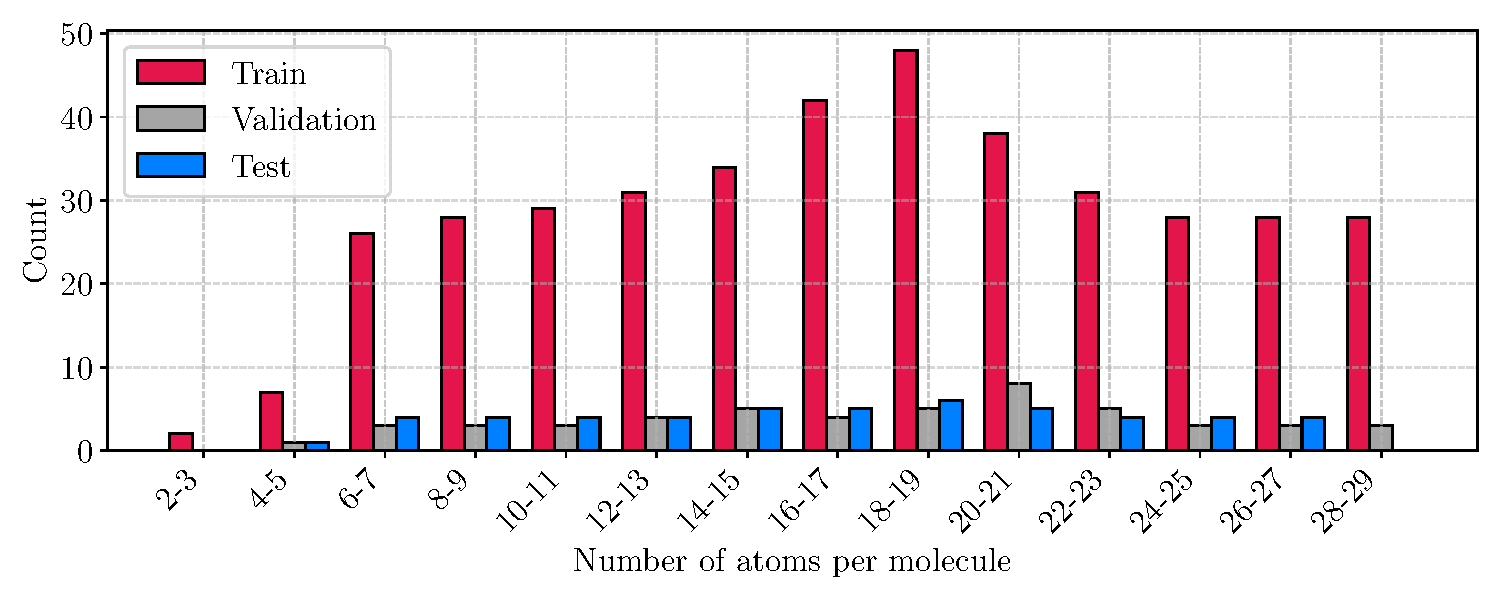
\includegraphics[width=0.85\textwidth]{../fig/application/strat_sample.pdf}
    \caption[Stratified sample of QM9 dataset]{Stratified sample of QM9 dataset by number of atoms per molecule for each set.}
    \label{fig:sample_QM9}
\end{figure}
We sample 500 molecules from the QM9 set in a stratified manner and additionally ensure ample representation for various molecule sizes. Therefore, compared to the actual distribution seen in \autoref{fig:method_qm9_overview}, the representation of molecules with 6 to 13 and 24 to 29 atoms per molecule is increased. This results in the distribution for the train, validation and test sets shown in \autoref{fig:sample_QM9}. Once again the train/validation/test split is 80/10/10 per cent. %BE spelling

Zero-shot predictions like those devised in the previous section are not possible on the full dataset due to missing encoders/decoders for \ch{N}, \ch{F} and their respective interaction blocks. Therefore, we will proceed directly to hyperparameter tuning. 
\subsection{Hyperparameter tuning}
\label{sec:qm9_full_isomers_hyp_tuning}
Network hyperparameter tuning was carried out in the same manner as above, except that the maximum number of training epochs was increased to 50 to accommodate the more diverse dataset. \autoref{tab:qm9_full_further_runs} shows the results for the ten best performing models.
\begin{table}[H]
    \centering
    \caption[GNN on full QM9 dataset sample with full matrix loss]{GNN on full QM9 dataset sample using full matrix loss and a maximum of 50 epochs to train. Metrics on test set and corresponding hyperparameter settings for the ten best performing networks in terms of iterations.}
    \label{tab:qm9_full_further_runs} 
    \resizebox{\textwidth}{!}{
        \begin{tabular}{l
                        S[table-format=2.1(2)]
                        S[table-format=-4(3)]
                        S[table-format=-1.3(2)]
                        S[table-format=1.3(1)]
                        S[table-format=1.4(1)]}
            \toprule
            Models                 & {Iterations / 1} & {$|\Delta E_\text{DFT}|$ / $\unit{\hartree}$}  & {$|\delta E_\text{DFT}|$ / 1} & {DIIS error / $\unit{\hartree}$} & {RMSE / 1} \\
            \midrule %Data from server run!
            $\text{GNN}^{\text{Full}}_\text{f. 0}$ & 12(2)     & 1.2(5.5) & 0.001(0.003)  & 0.034(0.011) & 0.009(0.003) \\ 
            $\text{GNN}^{\text{Full}}_\text{f. 1}$ & \B 12.0(17)    & 0.9(1.7) & 0.001(0.0011)  & 0.034(0.013) & \B 0.009(2) \\
            $\text{GNN}^{\text{Full}}_\text{f. 2}$ & 12.0(1.8) & 1.3(4.2) & 0.001(0.002)  & 0.035(0.011) & 0.009(0.003) \\
            $\text{GNN}^{\text{Full}}_\text{f. 3}$ & 12.0(1.9) & 1.6(2.7) & 0.0010(0.0017)  & 0.034(0.013) & 0.009(0.003) \\
            $\text{GNN}^{\text{Full}}_\text{f. 4}$ & 12.0(1.7) & 0.2(2.1) & 0.0002(0.0017)  & 0.044(0.048) & 0.009(0.003) \\
            $\text{GNN}^{\text{Full}}_\text{f. 5}$ & 12.0(1.8) & 0.3(2.7) & 0.000(0.002)  & \B 0.033(13) & 0.009(0.003) \\
            $\text{GNN}^{\text{Full}}_\text{f. 6}$ & 12(2)     & 0.3(1.9) & 0.0002(13)  & \B 0.033(13) & 0.009(0.003) \\
            $\text{GNN}^{\text{Full}}_\text{f. 7}$ & 12.1(1.6) & 0.7(2.5) & 0.0007(0.0019)  & 0.038(0.018) & 0.009(0.003) \\
            $\text{GNN}^{\text{Full}}_\text{f. 8}$ & 12(2)     & \B 0.1(1.9) & \B 0.0000(13)  & 0.035(0.012) & 0.009(0.003) \\
            $\text{GNN}^{\text{Full}}_\text{f. 9}$ & 12.1(1.8) & 1.3(2.3) & 0.0008(0.0013)  & 0.036(0.014) & 0.009(0.002) \\
            \bottomrule
        \end{tabular}
    }
   \resizebox{\textwidth}{!}{
    \begin{tabular}{lrrrrrrrrrr}
        \toprule
        Parameters & $\text{GNN}^{\text{Full}}_\text{f. 0}$ & $\text{GNN}^{\text{Full}}_\text{f. 1}$ & $\text{GNN}^{\text{Full}}_\text{f. 2}$ & $\text{GNN}^{\text{Full}}_\text{f. 3}$ & $\text{GNN}^{\text{Full}}_\text{f. 4}$ & $\text{GNN}^{\text{Full}}_\text{f. 5}$ & $\text{GNN}^{\text{Full}}_\text{f. 6}$ & $\text{GNN}^{\text{Full}}_\text{f. 7}$ & $\text{GNN}^{\text{Full}}_\text{f. 8}$ & $\text{GNN}^{\text{Full}}_\text{f. 9}$ \\
        \midrule
        Hidden dimension & 128 & 256 & 256 & 256 & 512 & 128 & 512 & 512 & 512 & 128 \\
        Batch size & 8 & 8 & 8 & 8 & 8 & 8 & 8 & 16 & 8 & 8 \\
        Data aug. factor & 4.00 & 1.00 & 1.00 & 1.00 & 1.00 & 2.00 & 4.00 & 3.00 & 1.00 & 2.00 \\
        Edge threshold & 3.40 & 2.58 & 3.98 & 3.21 & 2.85 & 3.29 & 3.27 & 2.72 & 3.44 & 2.30 \\
        Message passing steps & 4 & 5 & 3 & 2 & 4 & 2 & 3 & 3 & 2 & 4 \\
        Message Net dropout & 0.09 & 0.16 & 0.25 & 0.21 & 0.04 & 0.11 & 0.25 & 0.04 & 0.18 & 0.19 \\
        Message Net layers & 3 & 3 & 3 & 3 & 3 & 4 & 3 & 2 & 3 & 2 \\
        Learn rate & 6.90e-04 & 9.31e-04 & 1.61e-03 & 2.75e-04 & 8.03e-04 & 1.51e-04 & 1.26e-04 & 5.85e-04 & 1.09e-03 & 6.50e-04 \\
        Weight decay & 7.15e-05 & 5.46e-05 & 3.58e-05 & 4.69e-05 & 3.99e-04 & 6.06e-04 & 2.56e-04 & 1.45e-04 & 1.84e-05 & 1.74e-05 \\
        \bottomrule
    \end{tabular}
    }
\end{table}
Both the mean iteration count and its variability increased by about one cycle compared to the best-performing isomer models. Further analysis of iteration performance by molecule size revealed no clear correlation between atom count and the number of iterations to converge.
\subsection{Evaluation \& Conclusion}
\label{sec:qm9_full_isomers_conclusion}
Using our stratified QM9 sample, we show that our GNN implementation trained on just 400 molecules achieves lower SCF iteration counts than every other guessing scheme except \texttt{minao}. The greater chemical diversity in this subset leads to a uniformly higher standard deviation in cycle counts across all methods. \autoref{tab:qm9_full_test_overview} compares our top-performing GNN against the established guessing schemes.

Another notable finding emerges when contrasting the full dataset results for $\overline{P}$ with those from the isomer only runs. While the average number of iterations remained essentially unchanged, with only their spread increasing for the more diverse dataset, the DIIS error in the full dataset differs substantially from that in the isomer-only case. Furthermore, \texttt{minao} has the second highest DIIS error while simultaneously offering the fastest converging guess. Crucially, it once again underscores that DIIS error and iteration count are largely uncorrelated. 
\begin{table}[H]
    \centering
    \caption[Models compared to \textsc{PySCF} and $\overline{P}$ schemes - full QM9 dataset]{Comparison of GNN model with calculations employing \textsc{PySCF} and $\overline{P}$ guessing schemes on the full QM9 dataset. Here, $\overline{P}$ is computed blockwise across all molecules by averaging over each \ch{C}-\ch{C}, \ch{O}-\ch{H}, etc. block.
}
    \label{tab:qm9_full_test_overview}
    \resizebox{\textwidth}{!}{
        \begin{tabular}{l
                        S[table-format=2.1(1.1)]
                        S[table-format=-3.4(3)]
                        S[table-format=-1.6(1.1)]
                        S[table-format=1.3(1.1)]
                        S[table-format=1.4(1.1)]}
                        \toprule
                        Guessing schemes                 & {Iterations / 1} & {$|\Delta E_\text{DFT}|$ / $\unit{\hartree}$}  & {$|\delta E_\text{DFT}|$ / 1} & {DIIS error / $\unit{\hartree}$} & {RMSE / 1} \\
                        \midrule
                        $\text{GNN}^{\text{Full}}_\text{f. 1}$ & 12.0(17)& \B 0.9(1.7) & \B 0.001(11)  & 0.034(0.013) & \B 0.009(2) \\
                        $\overline{P}$                & 17(3)            & 40(19)     &  0.024(10)   & 0.042(6)  & 0.014(3)  \\
                        \texttt{1-e}                  & 19(3)            & 200(80)    &  0.13(4)     & 0.122(15) & 0.16(12)  \\
                        \texttt{vsap}                 & 14(2)            & 4.3(19)    &  0.0027(9)   & \B 0.024(3)  & 0.0106(14)\\
                        \texttt{atom}                 & 16(2)            & 10(5)      &  0.006(3)    & 0.039(7)  & 0.015(2)  \\
                        \texttt{minao}                & \B 11.1(11)& \B 2.4(8) & \B 0.0016(5)& 0.081(12) & 0.017(3)  \\
                        \bottomrule
                    \end{tabular}
    }
\end{table}
\chapter{Conclusion}
\label{chap:conclusion}

\appendix
\chapter{Appendix}
\label{sec:appendix}

\section{Initial guessing methods in \textsc{PySCF} \parencite{ref:pyscf}}
\label{sec:pyscf_initial_guessing_methods}
The \textsc{PySCF} package offers a variety of initial guessing methods for the density matrix for SCF calculations as described in the excerpt of the documentation \parencite{ref:pyscf_user_guide} bellow: 
\begin{itemize}
    \item \texttt{minao} (default): A superposition of atomic densities \parencite{ref:minao_sad1,ref:minao_sad2} technique, in which the guess is obtained by projecting the minimal basis of the first contracted functions in the cc-pVTZ or cc-pVTZ-PP basis set onto the orbital basis set, and then forming the density matrix. The guess orbitals are obtained by diagonalizing the Fock matrix that arises from the spin-restricted guess density.

    \item \texttt{1e}: The one-electron guess, also known as the core guess, obtains the guess orbitals from the diagonalisation of the core Hamiltonian, thereby ignoring all interelectronic interactions and the screening of nuclear charge. The 1e guess should only be used as a last resort, because it is so bad for molecular systems; see \parencite{ref:Lehtola2019}.

    \item \texttt{atom}: Superposition of atomic densities \parencite{ref:minao_sad1,ref:minao_sad2}. Employs spin-restricted atomic HF calculations that use spherically averaged fractional occupations with ground states determined by fully numerical calculations at the complete basis set limit in \parencite{ref:lethola_fully_numerical_atomic_potentials}.

    \item \texttt{huckel}: This is the parameter-free Hückel guess described in \parencite{ref:Lehtola2019}, which is based on on-the-fly atomic HF calculations performed analogously to \texttt{atom}. The spherically averaged atomic spin-restricted Hartree-Fock calculations yield a minimal basis of atomic orbitals and orbital energies, which are used to build a Hückel-type matrix that is diagonalized to obtain guess orbitals.

    \item \texttt{vsap}: Superposition of atomic potentials as described in \parencite{ref:Lehtola2019}. A sum of pre-tabulated, fully numerical atomic potentials determined with the approach of \parencite{ref:lethola_fully_numerical_atomic_potentials} is used to build a guess potential on a DFT quadrature grid; this potential is then used to obtain the orbitals. Note: this option is only available for DFT calculations in PySCF.
\end{itemize}



\section{Comments on second order Newton-solvers \& iterations}
\label{sec:notes_on_so_newton}
A second order Newton-solver essentially uses the Newton algorithm to converge an electron density by constructing density gradients $g$ and approximating the Hessian $H$ of the energy. The implementation in PySCF uses an outer macro loop which takes the newton steps and an inner loop which approximates the solution to the linearized Newton equation:
\[H \Delta x = -g\]
to obtain the update $\Delta x$ which is to be applied to the orbitals.\\

Faster convergence in terms of iterations was claimed by Schütt et al. for their neural network. \parencite{ref:schuett_unifying_2019} This prompted investigations on the \ch{C7H10O2} isomer set. Given our test set a comparable reduction of iterations from 1$^\text{st}$ order in \autoref{fig:dummy_iterations_qm9_isomers} to 2$^\text{nd}$ order\footnote{using PySCF's \texttt{newton\_ah} solver} in \autoref{fig:so_macro_iterations} can be seen. 

\begin{figure}[H]
    \centering
    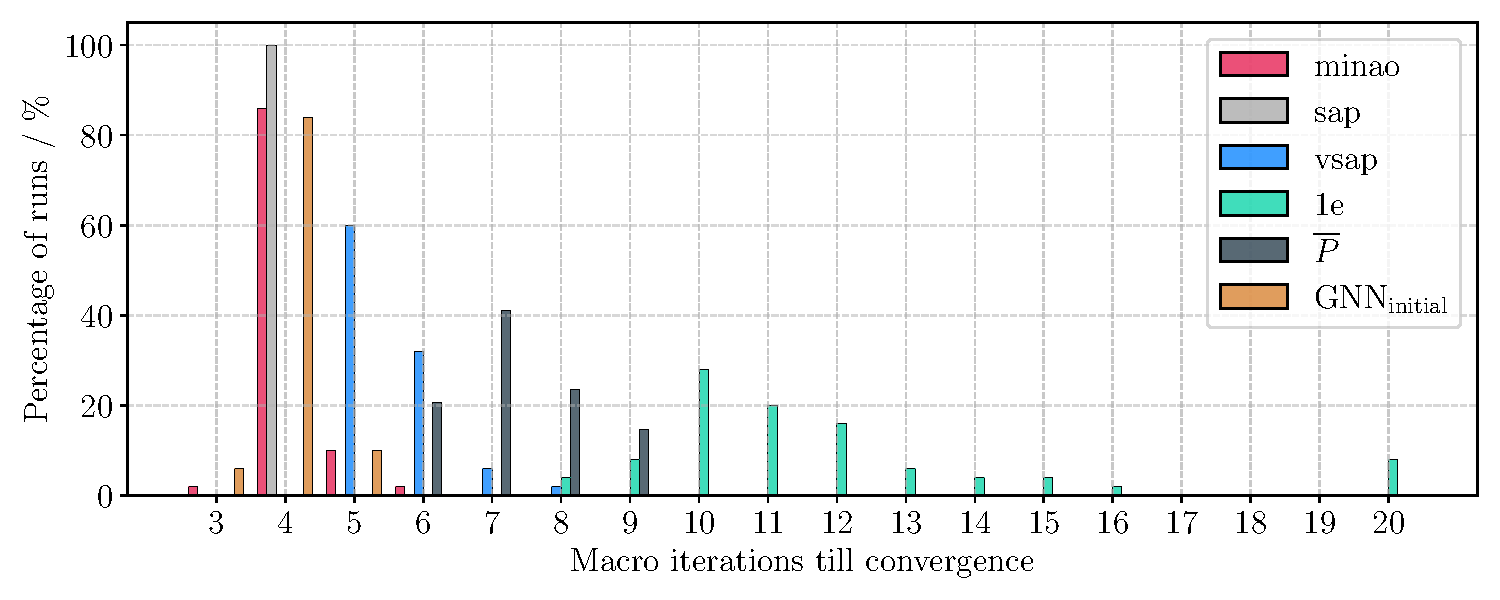
\includegraphics[width=\textwidth]{../fig/gnn/SO_0D_GNN_model_iteration_count_bar.pdf}
    \caption[Macro iterations till convergence distribution for QM9-isomers]{Macro iterations till convergence distribution for QM9-isomers for PySCF, $\overline{P}$ and GNN$_\text{initial}$ guesses. All entries with $\geq 20$ macro iterations are grouped at $20$.}
    \label{fig:so_macro_iterations}
\end{figure}
Yet this direct comparison is not a fair one. Contrary to DIIS, which builds the Fock matrix once per iteration, the Newton-solver repeatedly rebuilds the Fock matrix in it's inner loop. Summing all Fock matrix builds one obtains different behavior depicted in \autoref{fig:so_fock_build_iterations}.  
\begin{figure}[H]
    \centering
    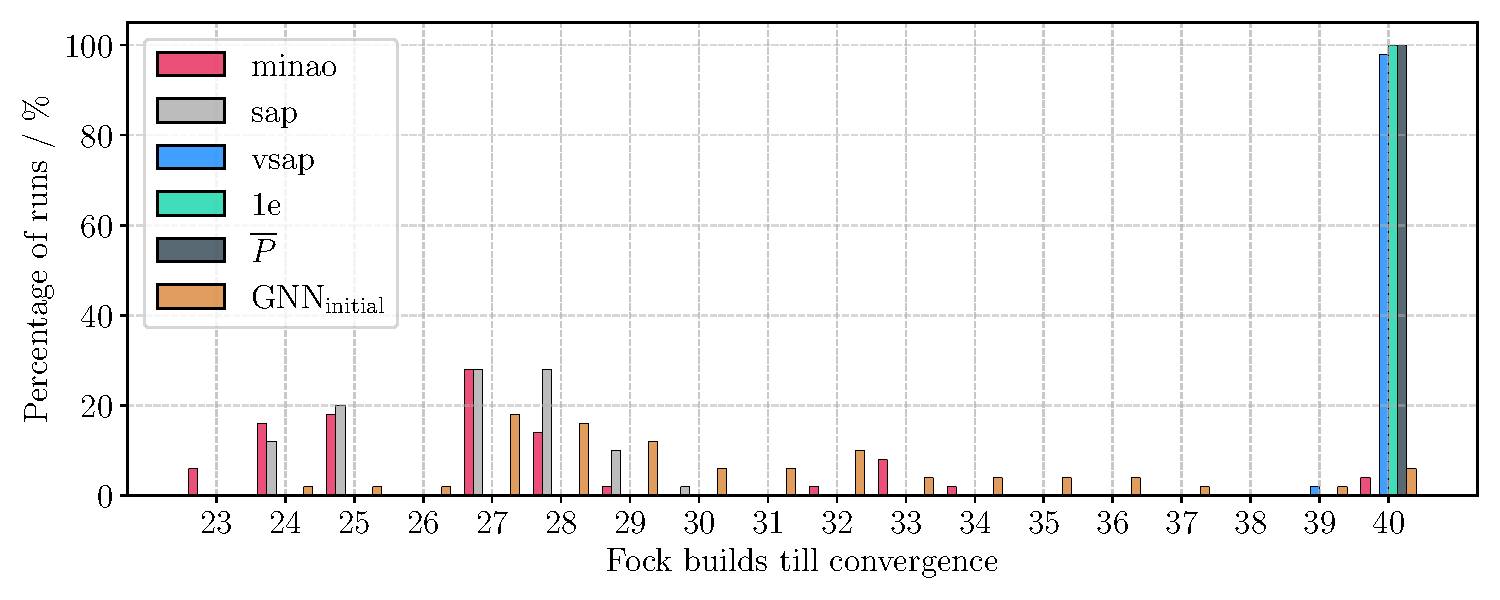
\includegraphics[width=\textwidth]{../fig/gnn/SO_0D_GNN_model_fock_build_count_bar.pdf}
    \caption[Fock matrix build count till convergence QM9-isomers]{Fock matrix build count till convergence for QM9-isomers for PySCF, $\overline{P}$ and GNN$_\text{initial}$ guesses. All entries with $\geq 40$ fock builds are grouped at $40$.}
    \label{fig:so_fock_build_iterations}
\end{figure}
Given this fact, one needs to be caution in making prediction regarding wall clock time of simulations from 'iteration` counts, especially for comparisons of different algorithms.

\section{Source Code \& Packages used}
\label{sec:source_code_packages}
%!TODO maybe add version here
The source code for this thesis was fully written in Python 3.11.11 and is made available upon request. \parencite{ref:python}\\

Models in \autoref{chap:fock_matrix_predictions} were trained using \textsc{scikit-learn} \parencite{ref:sk-learn} and \textsc{Tensorflow} \parencite{ref:tensorflow} with the \textsc{keras} frontend \parencite{ref:keras} and \textsc{kerastuner} for optimization \parencite{ref:kerastuner}. The GNN in \autoref{chap:gnn} was implemented using the \textsc{PyTorch Geometric} library \parencite{ref:PyTorchGeometric}. Hyperparameter optimization was performed using the \textsc{ray} library \parencite{ref:ray_tune}. Dataset handling was performed using a custom written \textsc{scf\_guess\_datasets} package which is available online \parencite{ref:milacher_scf_guess_datasets}. 

%--- INDEX and BIBLIOGRAPHY ----------------------------------------------------

%% Print List of Acronyms and Symbols  (optional)
%\printnoidxglossary[title={Notation}]
%\printnoidxglossary[type=acronym]
\newpage
\listoffigures
\vspace{-5mm}
\listoftables
\newpage
% Print bibliography and include it in the table of contents:
\printbibliography[heading=bibintoc]


\end{document}
